%!TEX root=../paper.tex

\chapter{WebRT: Smart Web Browser Runtime Optimizing for Energy-Efficiency}
\label{sec:runtime}

Today's mobile processors are becoming extremely heterogeneous. They often combine general-purpose cores that have different performance and energy characteristics~\cite{single-ISA} (e.g., asymmetric chip-multiprocessor architecture) with special-purpose domain-specific cores (e.g., \webcore). While the hardware upheaval promises performance and energy improvements for the mobile Web, current Web runtime systems are not designed to fully exploit the capability of the underlying hardware. The main bottleneck is that current runtime-architecture interface merely exposes the hardware as a monolithic sequential execution model to the runtime system while hiding many architecture-level details. Without having a full visibility of the hardware details, current Web runtimes often lead to energy-inefficient decisions or violate user QoS requirement.

To bridge the widening gap between the architecture complexity and the architecture-agnostic runtime system, I propose to enhance the existing runtime-architecture interface by exposing architecture details to the Web runtime. I specifically focus on the ACMP architecture~\cite{acmp,single-ISA} as the hardware substrate. ACMP is long known to provide a large performance-energy trade-off space, and is already widely used in today's mobile systems~\cite{big-little-future,exynos5biglittle}. I  quantitatively show that Web applications particularly benefit from the heterogeneity offered by the ACMP architecture to achieve an ideal balance between QoS experience and energy consumption (\Sect{sec:runtime:char}).

Leveraging the ACMP architecture, I propose \webrt, a Web runtime that minimizes energy while guaranteeing satisfactory user QoS experience by scheduling Web application executions using proper ACMP configurations. Particularly, I show that we must devise different optimization schemes according to the nature of different user interaction forms. To that end, I introduce a user-application interaction model called LTM. LTM captures three fundamental user interaction forms in mobile Web applications--Loading, Tapping, and Moving--and provides a framework for reasoning about different energy optimization strategies (\Sect{sec:runtime:overview}).

I then describe \webrt's two critical components. The first component is the webpage-aware scheduler that targets the loading (L) process of a Web application (\Sect{sec:runtime:load}), and the second component is the event-based scheduler that targets the touching (T) and moving (M) interactions (\Sect{sec:runtime:ebs}). Finally, I compare the contrast \webrt with prior work on software support for mobile Web (\Sect{sec:runtime:related}).

\section{Motivation: Energy-Delay Trade-off}
\label{sec:runtime:char}

%Our goal in this work is to meet the cut-off latency of webpage loading while minimizing the energy consumption under that constraint whenever possible.  In order to achieve that, we have to carefully balance the performance and energy consumption of webpage loading. Heterogeneous systems with big/little cores each with DVFS capabilities naturally enable a flexible balance between performance and energy due to a large scheduling space.  Different workloads, according to their behaviors, can be scheduled to different cores/frequencies to explore different trade-offs between performance and energy.

%Our goal in this work is to meet the cut-off latency of webpage loading while minimizing the energy consumption under that constraint whenever possible.

An ACMP consists of cores with different computation capabilities--often with different microarchitectures, such as big out-of-order cores and small in-order cores. Each core has a variety of frequency settings. Different core and frequency combinations provide a wide range performance and energy characteristics. The flexibility of an ACMP architecture to make trade-offs between performance and energy consumption leads us to answer a fundamental question: do Web applications benefit from an ACMP heterogeneous systems?  For example, can a processor lower the frequency for a simple webpage to consume less energy but still respect the QoS deadline? Can a webpage originally scheduled on an energy-consuming core be migrated to an energy-saving core without violating the QoS constraint?

We quantitatively answer this question using webpage loading as a case study. The same experimental methodology and conclusion also hold true for other types of interactions in mobile Web applications. We base our measurements and analysis on the 5,000 hottest webpages on the Internet ranked by \website{http://www.alexa.com/}. We show that different webpages require different core and frequency configurations to meet a given deadline of webpage loading while minimizing the energy. This suggests that ACMPs with both big and smalls core, each capable of performing DVFS, are strongly beneficial.

To demonstrate the benefits of such heterogeneous systems, we measure the webpage load time and energy consumption of the 5,000 webpages on the Cortex-A9 and A8 processors (See \Sect{sec:runtime:load:eval} for a detailed experimental setup). We sweep a total of seven configurations available on the big and little cores, i.e., Cortex-A9 with four DVFS settings and A8 with three DVFS settings, respectively. We begin our analysis with four webpages that represent the general trends that we observe (\Sect{sec:runtime:char:representative}), and we subsequently expand our analysis to include the comprehensive set of all webpages (\Sect{sec:runtime:char:comprehensive}).
% (\website{www.autoblog.com}, \website{www.newegg.com}, \website{www.adobe.com} and \website{www.baidu.com})

\subsection{Representative Analysis}
\label{sec:runtime:char:representative}

\Fig{fig:pareto} shows the energy versus delay plots for the four representative webpages. Assuming 3~seconds as the cut-off latency for webpage load~\cite{ThreeSecond}, the four webpages have different ideal core and frequency configurations to meet the cut-off while simultaneously minimizing the energy consumption. For example, \website{www.autoblog.com} is a complex website that has 4,235 nodes in the DOM tree, and it therefore requires the highest frequency on the big core to meet the cut-off latency. However, this configuration is overpumped for simpler websites such as \website{www.newegg.com} with 3,152 DOM tree nodes. It only requires 700~MHz of the big core. This suggests that some webpages can benefit from different frequencies in each processor's core.

\begin{figure}[p]
\centering
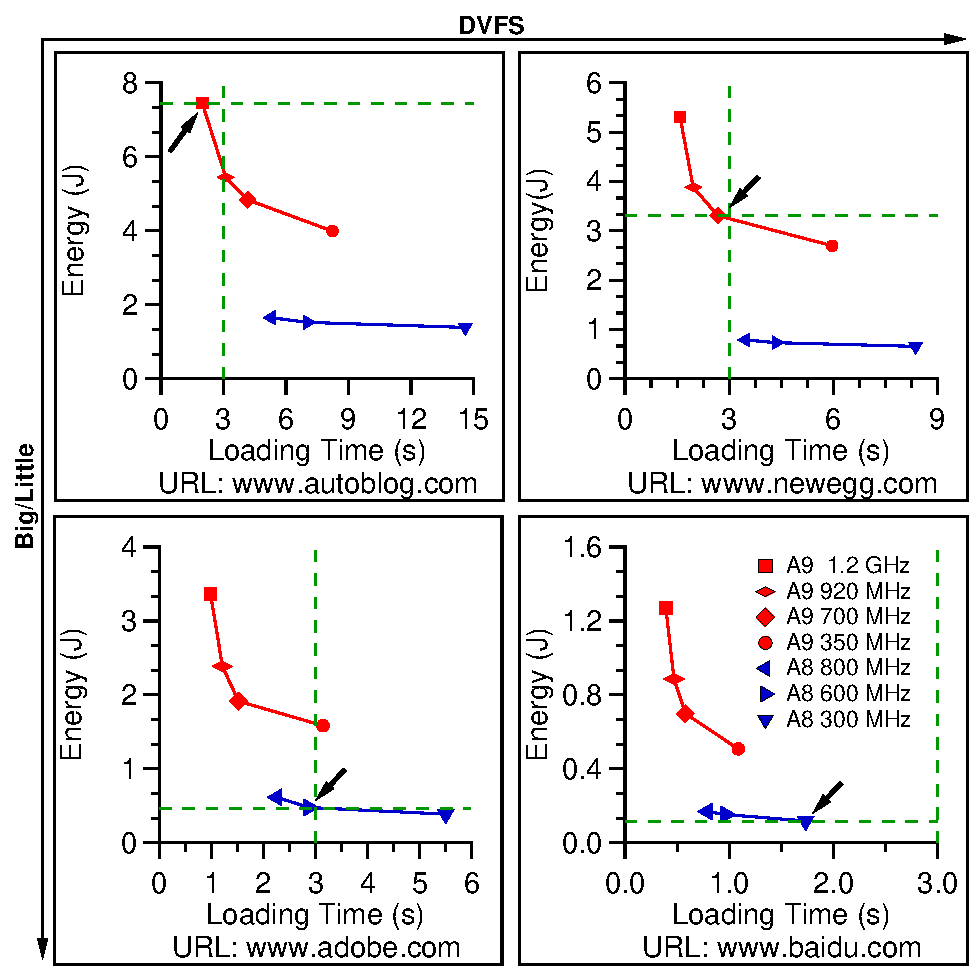
\includegraphics[trim=0 0 0 0, clip, width=\columnwidth]{pareto}
\caption{Webpages have different ideal execution configurations to meet the cut-off latency while consuming the least energy.}
\label{fig:pareto}
\end{figure}

In addition, some webpages can take advantage of scheduling between big/little cores. If only the big core is available, \website{www.adobe.com} can at best be loaded at 700~MHz. Instead, with the little core, the webpage can be loaded using 600~MHz, which still meets the cut-off latency but consumes 75\% less energy than 700~MHz on the big core. Similarly, \website{www.baidu.com} is a search engine website that has very concise content with less than 1~KB of images. It only requires the lowest frequency on the little core.

\subsection{Comprehensive Analysis}
\label{sec:runtime:char:comprehensive}

We extend our analysis to the full set of 5,000 webpages. \Fig{fig:conf-dist} shows the distribution of ideal core and frequency configurations for different cut-off latencies, ranging from 1~second to 10~seconds at 1~second intervals. Each region in \Fig{fig:conf-dist} represents the portion of webpages that are loaded at the corresponding architectural configuration with minimal energy consumption while still meeting the cut-off latency. We find a wide distribution of ideal configurations, indicating the benefits of a flexible baseline architecture that mixes big/little cores with different frequencies. 
%For example, if the cut-off latency is 1~s, the big core with its peak frequency can load 52.6\% of the webpages successfully while consuming the least amount of energy compared to all the other configurations.

\begin{figure}[t]
\centering
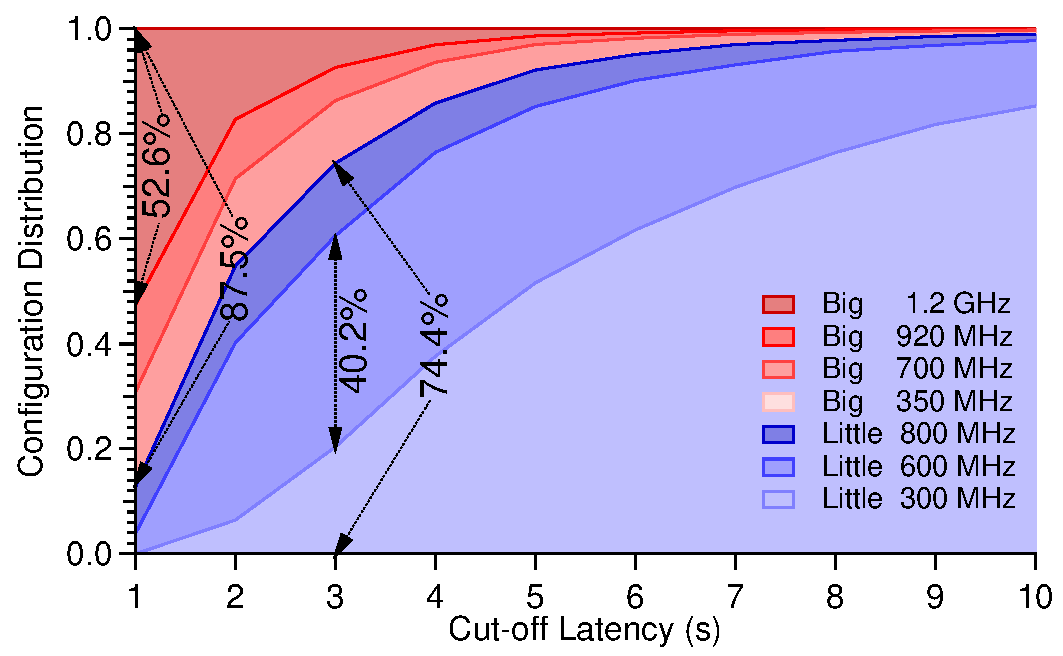
\includegraphics[trim=0 0 0 0, clip, width=.9\columnwidth]{conf_dist}
\caption{The distribution of ideal core and frequency configurations under different cut-off latencies.}
\label{fig:conf-dist}
\end{figure}

Assuming a tight 3~second cut-off latency~\cite{ThreeSecond}, a single core with a fixed frequency is insufficient for a wide spectrum of webpages.  The best single core with a fixed frequency is the little core with 600~MHz.  However, it can only load 40.2\% of the webpages within that latency constraint. Even a single core (big or little) with varying frequencies is insufficient. When we consider the little core with varying frequencies, only 74.4\% of webpages can be loaded within the cut-off latency. However, if we use a big core to load all the webpages, then the 74.4\% of webpages have suboptimal performance-energy trade-off. Furthermore, a simple heterogeneous system with both a big and little core but each with a fixed frequency may also cause suboptimal performance-energy trade-off for some webpages. Statistically, the best single-frequency configurations are 700~MHz on the big core and 600~MHz on the little core; yet, a heterogeneous system with only these two settings leads to ideal scheduling for only 52.1\% of the webpages.

Although 3~seconds is the typical cut-off latency on mobile systems, we also study the sensitivity of the ideal configuration distribution under other cut-off latencies. We find that varying cut-off demands also call for a flexible baseline architecture. As \Fig{fig:conf-dist} shows, no one particular configuration consistently performs well under varying cut-off latency requirements. For example, although relaxed cut-offs favor the little core, it is suboptimal for 87.5\% of the webpages under a tight 1~second constraint. Similarly, the big core, which performs very well under tight cut-offs, is overpumped under more relaxed constraints; it is only needed for about 3\% of webpages when the cut-off latency is 10~seconds.

%In conclusion, different webpages have different ideal core and frequency configurations, and can strongly benefit from a versatile heterogeneous system consisting of both big and little cores each capable of performing DVFS.
In summary, we find that different webpages require different ideal core and frequency settings to achieve the ideal balance between performance and energy-efficiency. Varying cut-off latencies also demand different ideal configurations. Therefore, we conclude that different webpages can strongly benefit from a versatile heterogeneous system consisting of both big and little cores each capable of performing DVFS.

\section{WebRT Overview}
\label{sec:runtime:overview}

An ACMP consists of cores with different microarchitectures, such as out-of-order and in-order. Each core has a variety of frequency settings. Different core and frequency combinations provide a large trade-off space between performance and energy. The objective of our ACMP-based \webrt is to find an ideal ACMP configuration (i.e., a $\langle core, frequency \rangle$ tuple) that minimizes the energy consumption while guaranteeing an acceptable responsive time when a user interaction happens.

%To systematically analyze user interactions in mobile Web applications, we introduce a simple conceptual model called LTM, which captures three primitive user interaction forms: loading application page (L), tapping the display (T), and moving a finger on the display (M). The three interactions cover a majority of human-computer interactions on mobile devices: every application requires a loading phase (L), and post-loading interactions on mobile devices are mostly performed in the form of finger tapping (T) or finger moving (M).

\begin{figure}[t]
  \centering
  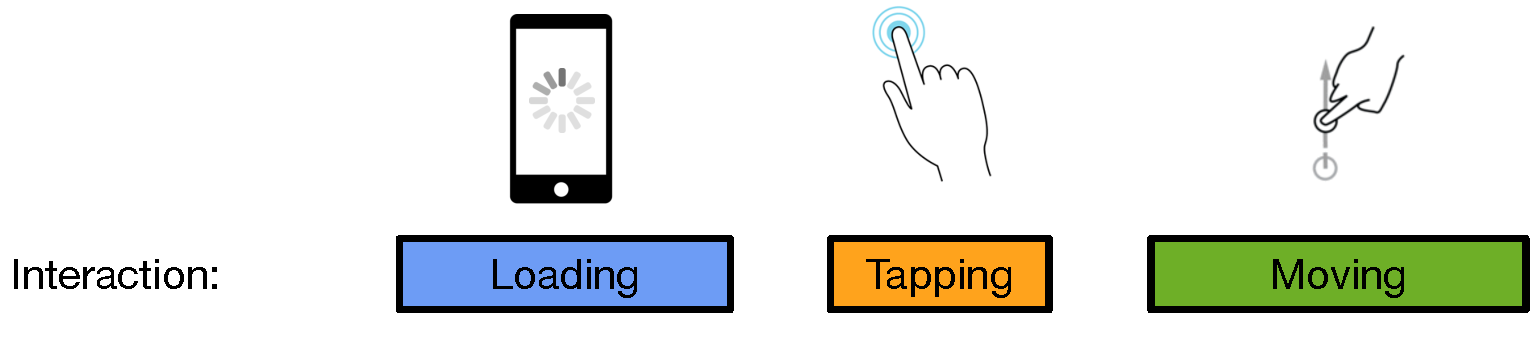
\includegraphics[trim=0 0 0 0, clip, width=.9\columnwidth]{interaction_model}
  \caption{The LTM (Loading-Tapping-Moving) user-application interaction model of mobile Web. LTM captures three primitive types of interaction: page loading, finger tapping, and finger moving. We use LTM as a framework to reason about user QoS experience.}
  \label{fig:interaction}
\end{figure}

To systematically analyze user interactions in mobile Web applications, we introduce a simple conceptual model called LTM, which captures three primitive user interaction forms in mobile Web applications: loading application page (L), tapping the display (T), and moving finger on the display (M). \Fig{fig:interaction} illustrates the LTM model.

The three interactions cover a majority of human-computer interactions on mobile devices. This is because every application requires a loading phase (L), and post-loading interactions on mobile devices are mostly performed in the form of finger tapping (T) or finger moving (M). The moving interaction in particular could be manifested in various ways, such as scrolling, swiping, or even drawing a picture. Internally, each user interaction is translated to one or more application event. For example, a tapping interaction is often translated to a \texttt{touchstart} and a \texttt{touchend} event, and a moving interaction can be translated to a \texttt{scroll} event or a \texttt{touchmove} event depending on context. In this paper, we focus on the following events that could be triggered by LTM interactions on a mobile device: \texttt{click}, \texttt{scroll}, \texttt{touchstart}, \texttt{touchend}, and \texttt{touchmove}. We do not consider events specific to desktops (e.g., \texttt{drag}, \texttt{mouseover}) that are generally not fired on mobile devices.

%Each event is bound to a DOM node with a callback function, which is executed when the event is triggered on the associated DOM node. The result of callback execution is fed into the Web browser rendering engine, which eventually paints the resulting frame(s) and updates the display. Frames are what users perceive as application's responses to their interactions, and thus determine the QoS experience.

The runtime optimization strategy for Loading is different from that for Touching and Moving. The fundamental difference is that Loading occurs only once per usage session while Touching and Moving interactions occur repetitively throughout the entire Web application usage session. As a result, it is possible to make the prediction for the Touching and Moving interactions based on the history information within the same usage session. For Loading, however, every application loading is likely different from the previous one, and as such we can not make predictions based on previous loadings of (potentially different) applications. Instead, we have to make prediction based on the particular content of a given Web application. I will discuss the \webrt component that targets the Loading in \Sect{sec:runtime:load} and the component that targets Touching and Moving interactions in \Sect{sec:runtime:ebs} separately.

\section{Webpage-aware Scheduling}
\label{sec:runtime:load}

In this section, I first show that it is possible to predict the webpage load time and energy consumption using merely webpage-inherent characteristics (\Sect{sec:runtime:load:model}). This prediction scheme had two advantages. First, it does not rely on any previous webpage loading history information and is based completely on each webpage's inherent characteristics. Second, the prediction is performed at the webpage parsing time which happens at the very beginning of the loading process, and as such allows enough time for energy optimizations.

Based on such predictions, we propose a webpage-aware scheduler as a \webrt component that predicts the ACMP configuration for webpage loading in order to minimize energy consumption while meeting a specified cut-off latency (\Sect{sec:runtime:load:sched}). Real hardware and software measurements show that against a performance-oriented hardware strategy, the webpage-aware scheduler achieves 83.0\% energy savings while violating the cut-off latency for only 4.1\% more webpages. Compared with a more intelligent, on-demand OS DVFS scheduler, the mechanism achieves an additional 8.6\% energy savings along with a 4.0\% performance improvement~(\Sect{sec:runtime:load:eval}).

\subsection{Performance and Energy Modeling}
\label{sec:runtime:load:model}

%!TEX root=../../paper.tex

\begin{table}[t]
\centering
\captionsetup{width=.9\columnwidth}
\renewcommand*{\arraystretch}{1.4}
\renewcommand*{\tabcolsep}{15pt}
\resizebox{.9\columnwidth}{!}{
\begin{tabular}{ll}
\toprule[0.15em]
\multicolumn{1}{l}{\bigstrut\textbf{Category}} & \multicolumn{1}{l}{\textbf{Model Predictors}}\\
\midrule[0.05em]
\multicolumn{1}{l}{\multirow{3}{*}{Webpage primitive: HTML}}
                &       Number of each tag \\
                &       Number of each attribute\\
                &       Number of DOM tree node\\
\midrule[0.05em]
\multicolumn{1}{l}{\multirow{3}{*}{Webpage primitive: CSS}}
                &       Number of rules \\
                &       Number of each selector pattern\\
                &       Number of each property \\
\midrule[0.05em]
\multicolumn{1}{l}{\multirow{2}{*}{Content-dependent}}
                &       Total image size \\
                &       Total webpage size \\
\bottomrule[0.15em]
\end{tabular}
}
\caption{Model Predictors}
\label{tab:feat_list}
\end{table}



\paragraph{Model Derivation} We find that regression models provide sufficient accuracy to predict the webpage load time and energy consumption. A regression model is a mathematical function between a set of predictors and a response. Within our context, the response is either the webpage's load time or energy consumption in loading the webpage. The predictors are a set of webpage characteristics. The linear regression model models a webpage's load time and energy consumption (responses) as a linear combination of various webpage characteristics (predictors), formulated as: $y = \beta_0 + \sum_{i=1}^{p} x_i \beta_i$ where \textit{y} denotes the response, \textit{$x = x_{1},...,x_{p}$} denote \textit{p} predictors, and \textit{$\beta = \beta_{0},...,\beta_{p}$} denote corresponding coefficients of each predictor. The \textit{least squares method} is used to identify the best-fitting $\beta$ that minimizes the residual sum of squares (RSS)~\cite{ESL}.

We consider two types of predictors. The first type includes the \textit{webpage-inherent} primitives such as the number of HTML tags. These primitives have show strong inter-webpage differences, and as such have a strong influence on the load time and energy consumption. In addition, we must also consider the impact of \textit{content-dependent} characteristics such as image size and the total size of a webpage. These characteristics are coarse-grained metrics that are independent of webpage structures but which influence the load time and energy of rendering. A media website is a classic example where content-dependent characteristics are dominant. For example, a news website, such as \website{www.bbc.com}, has a relatively stable appearance. Its structural layout (i.e., HTML) and style (i.e., CSS) do not change frequently. However, the website's content is changing daily to keep up with the latest breaking news. For instance, they are constantly updating images, and image sizes have a significant impact on the webpage load time. In our measurement we observe a 4X load time difference between a 200~KB and 50~KB image. Therefore, it is necessary to consider both webpage-primitive and content-dependent characteristics for modeling the load time and energy consumption of webpage load.

We summarize these features in \Tbl{tab:feat_list}. In total, we consider 376 predictors. We require a number of sampling observations to construct the regression models. In total, we obtain 2,500 sampling observations, for which we measure both webpage load time and energy consumption simultaneously on the Cortex-A9 processor running at 1.2 GHz.
 
\paragraph{Model Specification and Refinement} We apply various techniques to mitigate overfitting and capture predictor-response nonlinearity to achieve high prediction accuracy. We use R~\cite{R} and its \textit{glmnet} and \textit{rms} packages for all analysis.

We consider a large number of predictors (376) relative to the number of observations (2,500). This is known to produce predictions that result in overfitting~\cite{ESL}. We mitigate this, to the first order, by eliminating predictors that are less correlated to the response. We test the predictor/response correlation strength by calculating the squared correlation coefficient ($\rho^2$) between each predictor variable and observed load time and energy. \Fig{fig:pred-strength} shows the seven most-correlated predictors. For both load time and energy, we find the number of DOM tree nodes (\textsf{\#nodes}) is the most-correlated webpage primitive because it heuristically captures the webpage structure's complexity. Also, both image size and the total webpage size are also correlated because they capture the webpage content. We only select predictors with $\rho^2$ greater than 0.01.

\begin{figure}[t]
\subfloat[Predictor-response correlation.]{
  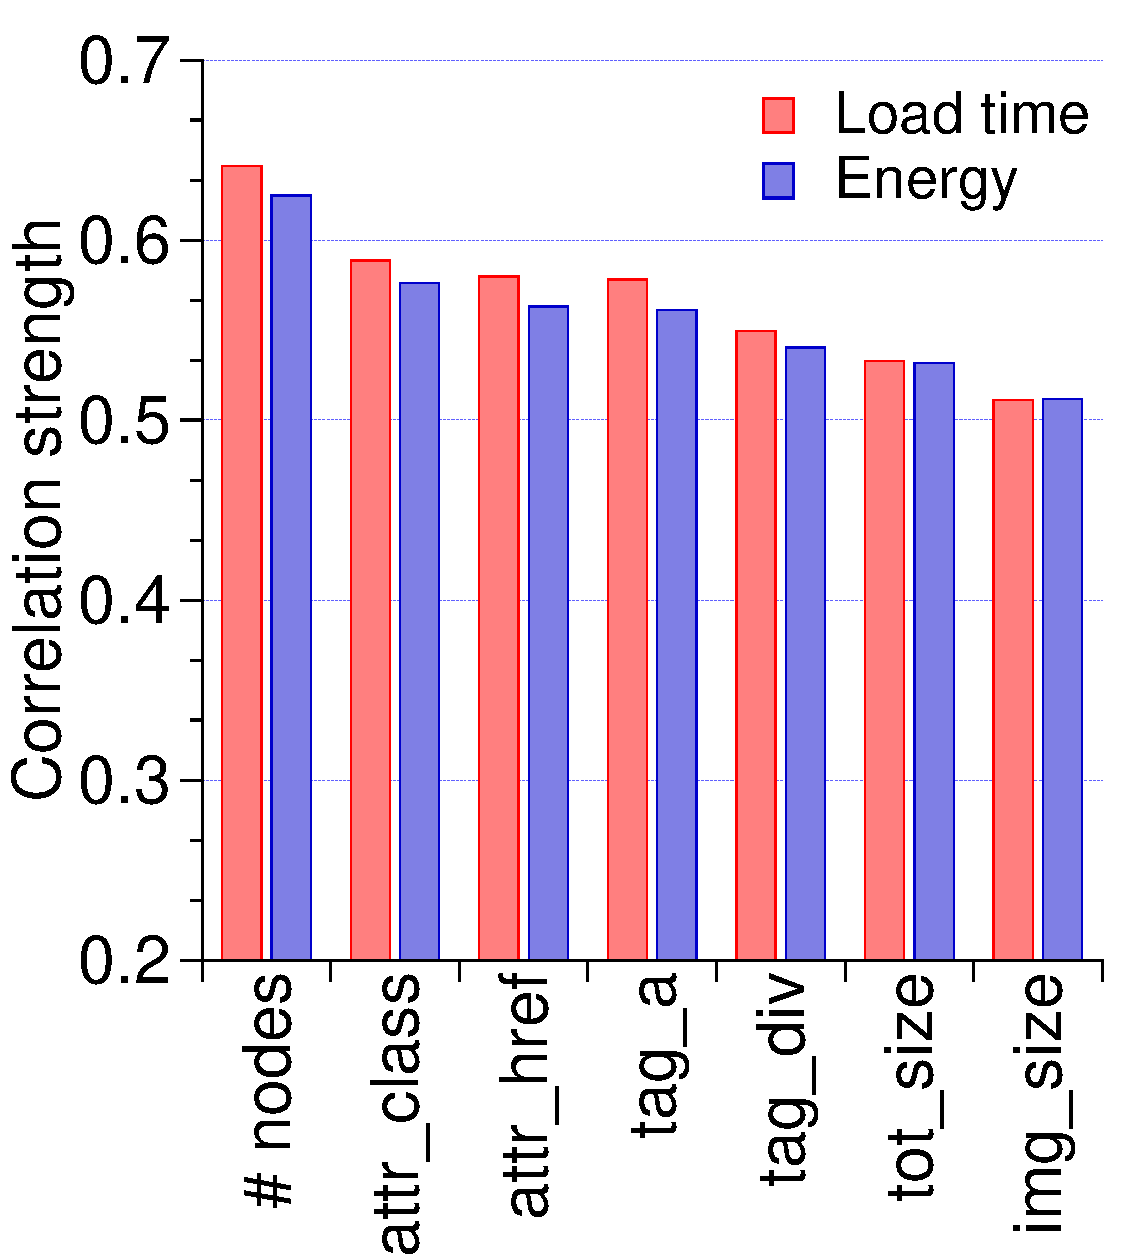
\includegraphics[trim=0 0 0 0, clip, width=.45\columnwidth]{pred-strength-new}
\label{fig:pred-strength}
}
\hspace*{1pt}
\subfloat[Predictor self-correlation.]{
  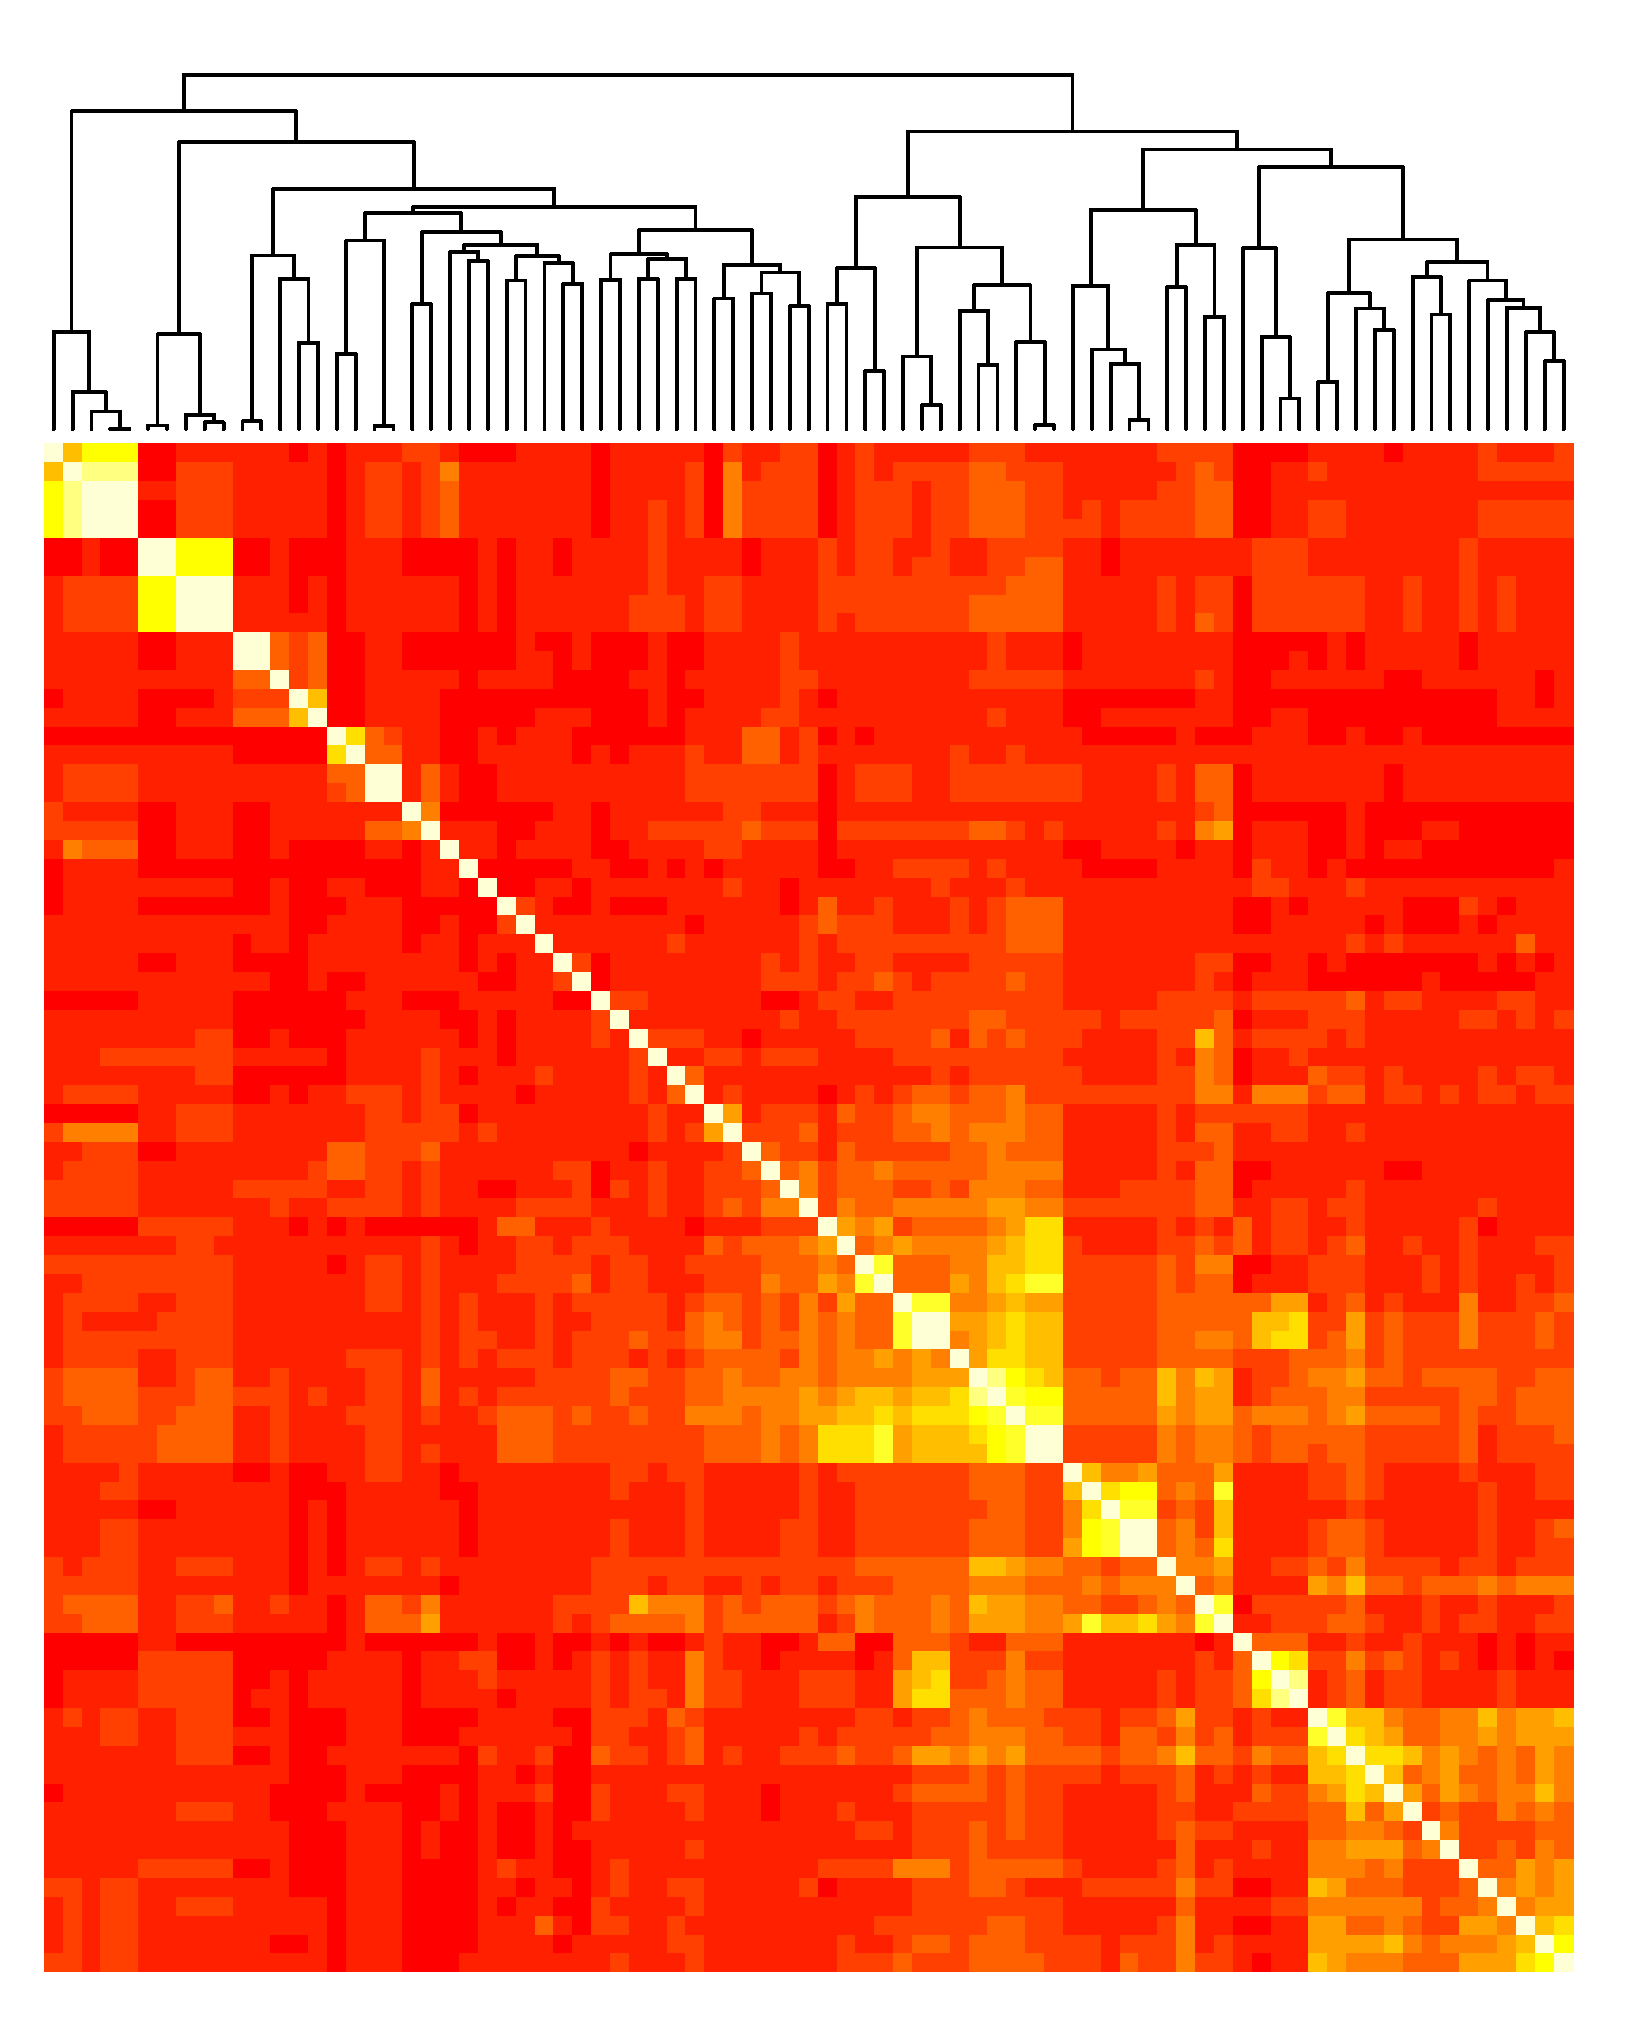
\includegraphics[trim=0 0 0 0, clip, width=.45\columnwidth]{all_cor-new}
\label{fig:all_cor}
} 
\caption{Predictor correlations.}
\label{fig:pred_cor}
\end{figure}

We further minimize overfitting by pruning features that are correlated to each other.  We test the correlation across predictors left after predictor strength test.  The correlation matrix is shown as a heatmap in \Fig{fig:all_cor}. The intensity of a point in the heatmap is proportional to the magnitude of the correlation coefficient between two predictors. The height of the branches in the dendrogram quantifies this magnitude.

In general, we find two types of correlation: inherent correlation and imposed correlation. Several HTML tags and attributes are functionally defined symbiotically and most often used together, exemplifying the inherent correlation. For example, the $<$\texttt{form}$>$ tag describes a form in the webpage, and the \texttt{action} attribute specifies where to submit the form. These two predictors are almost synchronized with each other, suggesting redundancy. Similar examples are the $<$\texttt{a}$>$ tag and the \texttt{href} attributes, which are defined to specify an external hypertext link. Some other predictors do not bear such an inherent relationship, but web developers use them together to describe related information, such as an image's width and height. For example, CSS properties \texttt{height} and \texttt{width} are highly correlated. The descendant selector pattern and class selector pattern also show heavy correlation for this reason.

Furthermore, it is unlikely that the true relationship between the response and all predictors is strictly linear as assumed by simple linear models.  One effective method to model nonlinearity is to fit data with \textit{restricted spline} functions that are piecewise polynomial functions but which force linear fitting beyond the first and last knots~\cite{ESL}.

\subsection{Model Evaluation}
\label{sec:model-eval}

To validate the model, we obtain 2,500 observations in addition to the 2,500 observations used for deriving the model. We incrementally evaluate the effect of various refinement techniques described previously by comparing the accuracy of three regression models. First, we evaluate a basic linear regression (L) model that prunes less-significant predictors. Second, we evaluate linear regression with regularization (R) that further prunes predictors correlated with each other. Third, we evaluate a restricted cubic spline-based (RCS) model using pruned features, which captures the nonlinear relationship between predictors and responses. Of all three models, RCS performs best at predicting both load time and energy. We show all three models for completeness of evaluation.

\paragraph{Performance model} The basic linear regression model (L) has a median and mean error rate of 25.8\% and 32.8\%, respectively, indicating a less-desirable prediction. The regularization-based model (R) reduces the median and mean error rate to 11.5\% and 13.6\%, respectively, due to more aggressive predictor pruning. Restricted cubic spline (RCS) modeling predicts the best, with the median and mean error rate of only 5.7\% and 7.5\% due to its capability of capturing more complex relationships between predictors and responses.

We also assess the distribution or prediction errors. \Fig{fig:perf_cdf} shows the results by presenting the cumulative distribution of the error for three modeling methods. Each ($x$, $y$) point in the graph corresponds to the portion of pages ($y$) that are at or below a particular error rate ($x$). Owing to overfitting, L predicts very accurately for a few webpages, but lacks the capability to be generally applicable to a large range of webpages.  As a result, L can only predict 20.0\% of the webpages within 10\% error. In contrast, R mitigates overfitting due to aggressive pruning, and predicts 44.6\% of the webpages within 10\% error. Finally, RCS further captures the nonlinear relationship, and therefore can predict 73.0\% of the webpages within 10\% error, and 94.0\% webpages within 20\% error.

\paragraph{Energy Model} Similar to the load time model, the RCS-based model performs the best, with the median error rate of 6.4\% (mean of 8.2\%), dropping from the median of 12.3\% and 27.1\% for R and L, respectively. \Fig{fig:energy_cdf} shows the cumulative distribution of the error for three modeling methods. For reasons explained earlier, RCS can predict 70.0\% of the webpages within 10\% error (91.8\% within 20\% error), improving from 41.7\% and 18.7\% of R and L, respectively.

\begin{figure}[t]
\subfloat[Load time model.]{
    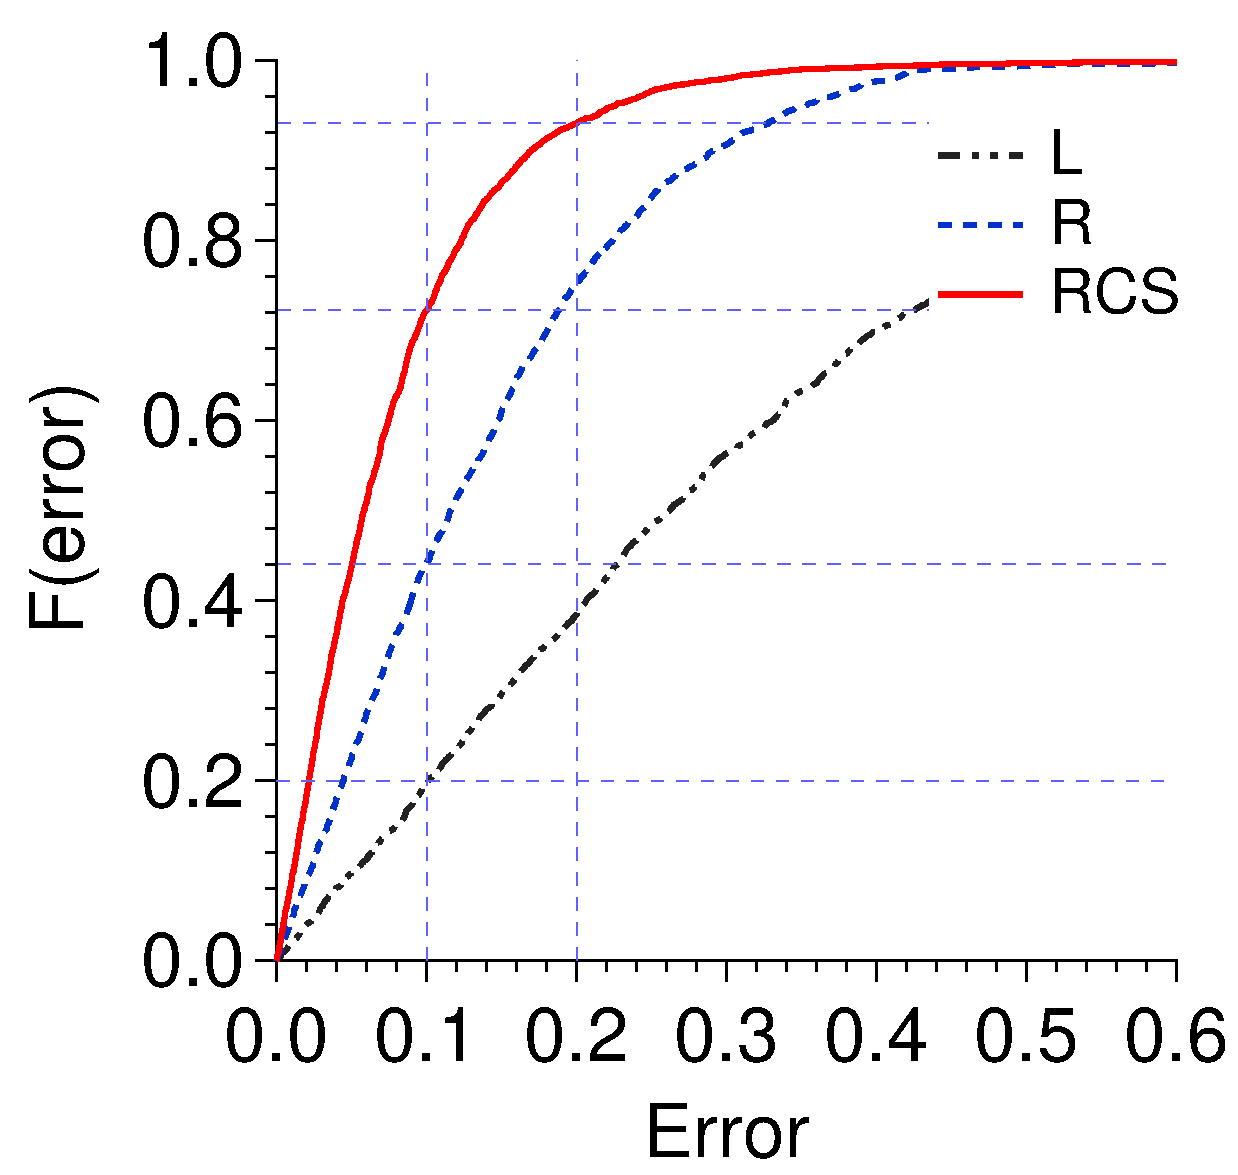
\includegraphics[trim=0 0 0 0, clip, width=.45\columnwidth]{perf_cdf}
\label{fig:perf_cdf}
}
\hspace*{15pt}
\subfloat[Energy model.]{
    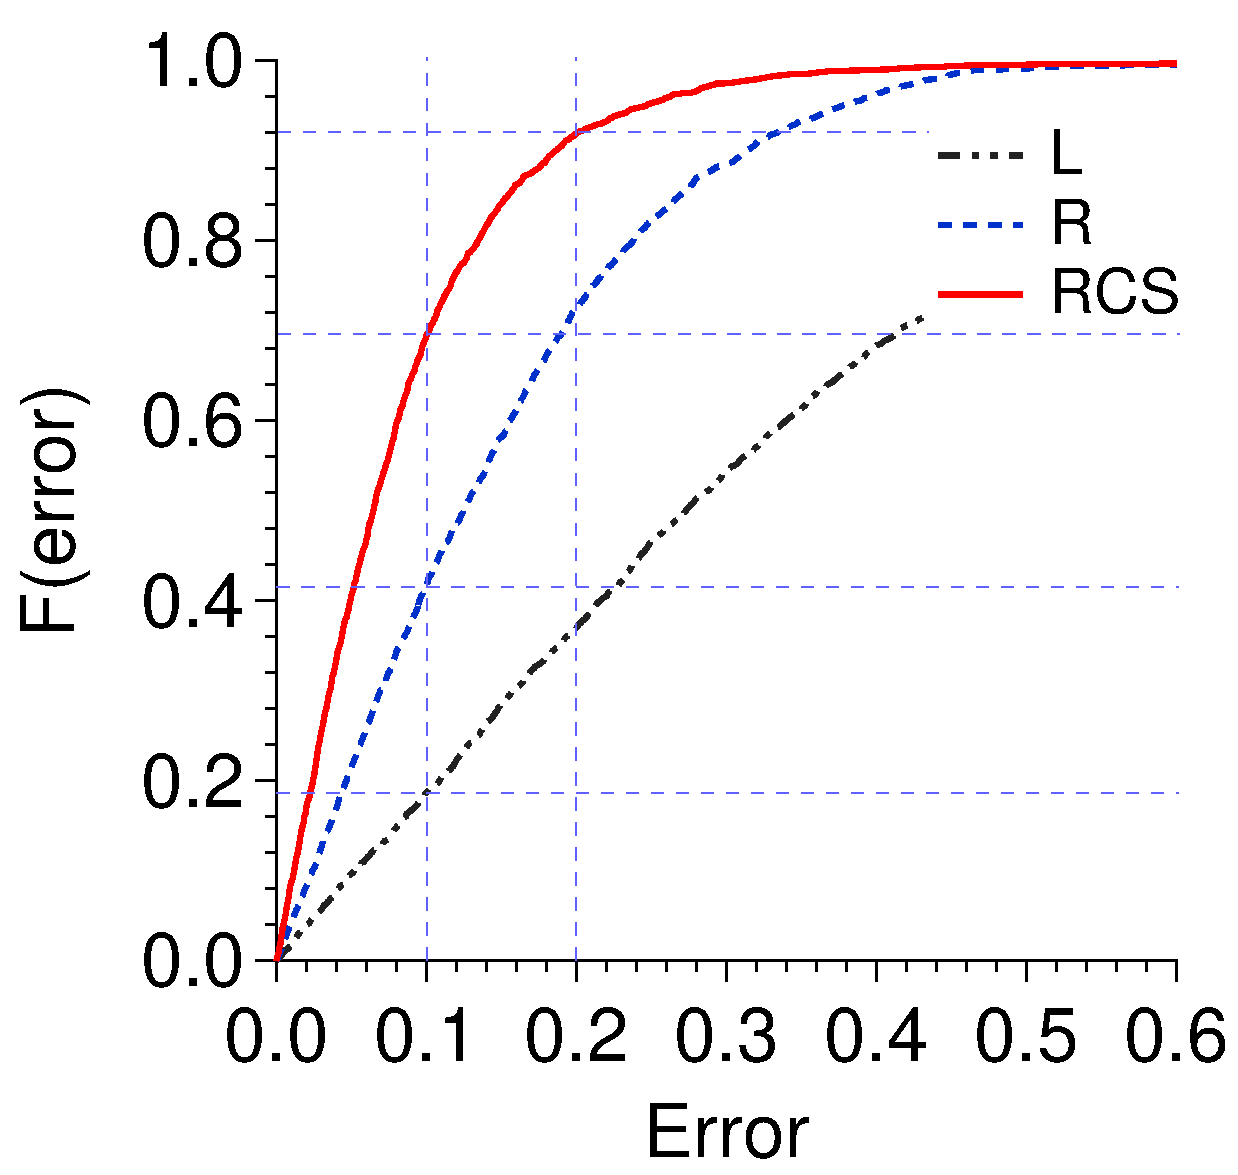
\includegraphics[trim=0 0 0 0, clip, width=.45\columnwidth]{energy_cdf}
\label{fig:energy_cdf}
} 
\caption{CDF of prediction errors.}
\label{fig:model_eval}
\end{figure}

\subsection{Scheduler Implementation}
\label{sec:runtime:load:sched}

\paragraph{Scheduler} During the parsing stage, which takes \textless 1\% of the total execution time, the webpage-aware scheduler extracts webpage characteristics, and feeds them into the prediction models to estimate the webpage load time and energy consumption under different core and frequency configurations.  On the basis of these predictions, the scheduler then identifies the configuration (if possible) that meets the cut-off latency with minimal energy consumption. If no such configuration is found, the webpage is scheduled to the big core with the highest frequency for the best possible performance.

\paragraph{Scheduling Overhead} We consider two major scheduling overheads: prediction and configuration transitioning. Prediction occurs very rapidly (\textless 3~milliseconds on the Cortex-A9 under 1.2~GHz). Moreover, prediction is interleaved with the parsing stage of the rendering engine. As parsing in modern browsers is highly optimized (e.g., asynchronous with the other processing), the prediction overhead is insignificant. On the basis of our measurements, we assume a constant overhead of 5~milliseconds.

Transitioning between hardware configurations involves the penalty of migrating tasks between big/little cores and/or frequency scaling overhead. The major overhead source of task migration is context switch, i.e. (re)storing architecture state such as register files and configuration registers, as well as warming up the private L1/L2 caches (assuming cache coherency between the last-level cache (LLC) of big and little cores). We assume a constant overhead of 20~milliseconds for state (re)storing per context switch, as indicated for the ARM big.LITTLE system~\cite{big.little}. For private cache warmup penalty, prior work shows that performance often improves when private LLCs of big and little cores are powered on together~\cite{PIE}. Thus, we ignore the warmup penalty. Also, prior work suggested that the power overhead of task migration is <~0.75\%~\cite{tm}. Thus, we do not consider the additional energy consumption of our scheduling mechanism.

For frequency scaling, we assume 0.3~milliseconds as the overhead. The Linux kernel uses this value on both the Cortex-A9 and A8 systems. This value takes into account both hardware (i.e., voltage regulator module switching frequency) and software overhead (i.e., privilege-level switching overhead for the frequency change request). In our evaluation, since we do not know which configuration the web browser is currently running in, we conservatively consider both the configuration transitioning overhead and the frequency scaling overhead at every scheduling point.

\subsection{Evaluation}
\label{sec:runtime:load:eval}

\paragraph{Energy savings} We compare the webpage-aware scheduling mechanism against an intelligent synthesized OS scheduler that performs on-demand DVFS on a heterogeneous system. The OS scheduler scales the frequency during a webpage load based on simple heuristics of system utilization~\cite{OS_DVFS1,OS_DVFS2}. It samples the CPU usage at a certain period and scales up the frequency if the average CPU usage in the previous sampling period is above a preset threshold, and vice versa. Because no Linux scheduler can yet perform heterogeneous scheduling across big/little cores, we synthesize such a scheduler by running the webpages under the ``on-demand'' cpufreq-governor~\cite{ondemand} on the big core and the little core, individually, and then choose the better result.

We compare the two scheduling techniques with a baseline strategy that consistently yields the best performance. We determine such a baseline by assessing the performance of all the different core and frequency configurations. \Fig{fig:cutoff_cdf} shows the cumulative distribution of webpage load time under each configuration. Each ($x$, $y$) point in the figure represents the portion of webpages ($y$) loaded within a certain delay ($x$). The big core with the peak frequency (1.2~GHz) achieves the best overall performance. It can load 96.5\% of the webpages within 3~seconds. As the frequency and core capability degrade, fewer webpages can be loaded within the same cut-off latency. Therefore, we choose the big core~(A9) with its peak frequency~(1.2~GHz) as the high-performance baseline.

\begin{figure}[t]
\centering
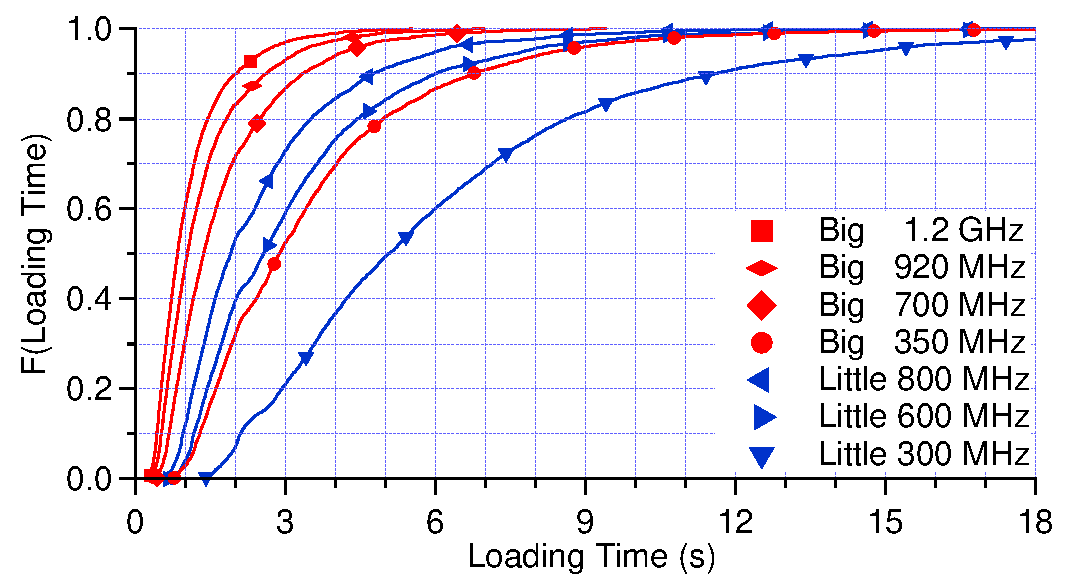
\includegraphics[trim=0 0 0 0, clip, width=.9\columnwidth]{cutoff_cdf}
\caption{CDF of webpage load time under different configurations.}
\label{fig:cutoff_cdf}
\end{figure}

We evaluate the same 2,500 webpages that we used to assess the accuracy of the regression models. Assuming a 3~second cut-off latency, \Fig{fig:results_energy} shows the boxplot of per-webpage energy savings under the webpage-aware and OS schedulers against the high-performance mode. Both schedulers achieve significant energy savings over the high-performance baseline, with a (geometric) average of 83.6\% and 83.0\%, respectively. This is because both schedulers can schedule webpages to the lower power core or lower frequency.

\begin{figure}[t]
\subfloat[Distribution of per webpage energy saving against the baseline.]{
    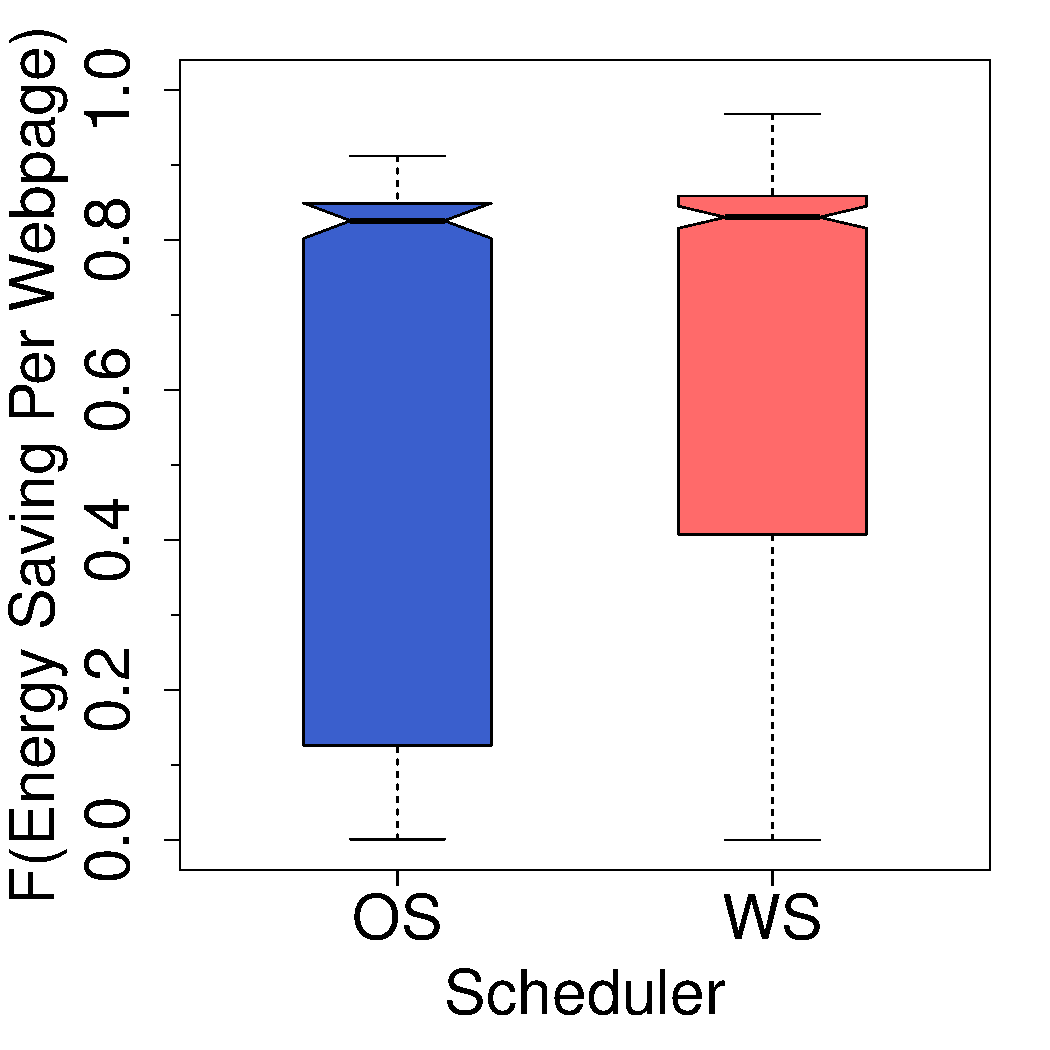
\includegraphics[trim=0 0 0 0, clip, width=.45\columnwidth]{boxplot}
\label{fig:results_energy}
}
\hspace*{15pt}
\subfloat[Number of webpages that load under the strict cut-off latency of 3~seconds.]{
    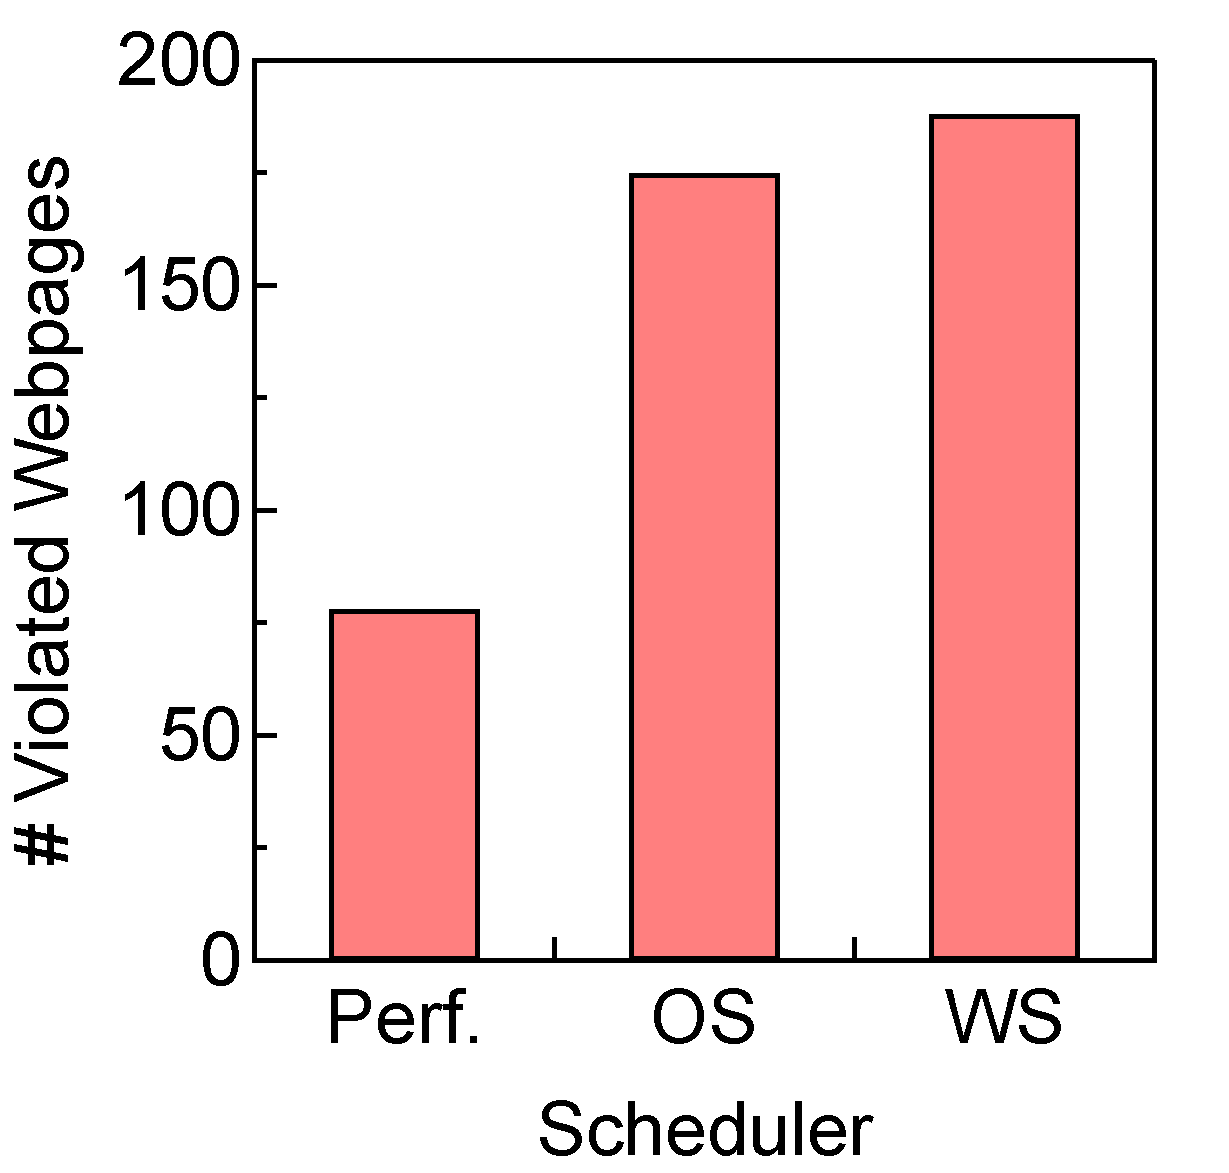
\includegraphics[trim=0 0 0 0, clip, width=.45\columnwidth]{results_cutoff}
\label{fig:results_cutoff}
} 
\caption{Evaluation of different scheduling strategies.}
\label{fig:sched_results}
\end{figure}

The webpage-aware scheduler has a denser energy-saving distribution toward 100\% than the OS scheduler. This indicates that generally the webpage-aware scheduler achieves higher energy savings. \Fig{fig:webpage-aware} shows the histogram of per-webpage relative energy of the webpage-aware scheduler to the OS scheduler. The webpage-aware scheduler saves energy for about 80\% of the webpages. There are several webpages that are mis-scheduled onto the big core that could have met the cut-off latency with the little core. These webpages consume much higher energy under the webpage-aware scheduler than the OS scheduler (\textgreater 2$X$ in~\Fig{fig:webpage-aware}).  On average, the webpage-aware scheduler reduces energy consumption by 8.6\% compared with the OS scheduler.

\paragraph{Performance impact} Both the OS scheduler and the webpage-aware scheduler trade performance for better energy savings compared with the performance mode. We evaluate their behaviors more critically using the number of webpages that violate the cut-off latency under their operations. This data is shown in \Fig{fig:results_cutoff}. The performance mode violates only 3.5\% of the webpages with a 3~second cut-off latency because it always operates at peak computational capability. Both of the software schedulers perform slightly worse. Our mechanism, the webpage-aware scheduler, results in 7.6\% violations, which is only 0.6\% worse than the OS scheduler. However, on (geometric) average, our mechanism loads webpages 4.0\% faster than the OS scheduler.

\paragraph{Cut-off sensitivity} To assess the webpage-aware scheduler under variable user demands and mobile device conditions, we also experiment with different cut-off latencies. For example, when the end user requests faster webpage load at 2~seconds, the mechanism achieves 7.3\% energy savings over the OS scheduler while violating 4\% fewer webpages. In a battery conservation mode where performance is less critical and the cut-off latency is relaxed to 10~seconds, the webpage-aware scheduler achieves 11.8\% energy savings compared with the OS scheduler while exceeding the cut-off latency for only 0.02\% webpages in total. We conclude that the webpage-aware scheduler is flexible to changing user requirements.

\paragraph{Prediction Accuracy} Scheduling effectiveness relies on the load time and energy prediction accuracy. We study the impact of the prediction accuracy by comparing webpage-aware scheduling with an Oracle scheduler that assumes perfect prediction under the 3~second cut-off latency. There are two types of misprediction: over-prediction causes webpages to load on a more powerful configuration that consumes more energy than the ideal one but does not cause cut-off violation; under-prediction loads webpages on a weaker configuration that consumes less energy but violates the cut-off constraint.  Our models lead to 10\% over-prediction and 4.1\% under-prediction. Compared with the Oracle scheduler, the webpage-aware scheduler results in 4.1\% cut-off violation but ``conserves'' 9.7\% energy.

\paragraph{Analysis} The advantage of the webpage-aware scheduler lies in its awareness of the webpages characteristics and the cut-off latency. As a result, it predicts and chooses a proper, albeit fixed, configuration for each webpage. In contrast, the OS scheduler's DVFS decision is based on the system utilization, which has no direct correlation with the webpage characteristics/cut-off latency and is sensitive to other system activities. Therefore, it may lead to a suboptimal performance-energy trade-off or even miss the cut-off constraint.

For example, when loading \website{www.newegg.com} (top-right in~\Fig{fig:pareto}) under the OS scheduler, we find that the CPU usage on the big core reaches above 95\% for around 40\% of the time and (unnecessarily) incurs peak frequency (i.e. 1.2~GHz).  When in fact, the big core with 720~MHz chosen by the webpage-aware scheduler is sufficient  to meet the 3-second cut-off latency, achieving 20\% energy savings compared with the OS scheduler in our experiments.

However, the flexibility to scale the frequency while loading a webpage sometimes allows the OS scheduler to exploit the marginal value of energy, i.e. a slight increase in energy (through frequency scaling) can bring the webpage back within the cut-off latency that would have been missed if the webpage were loaded using a lower frequency.

For example, \website{www.autoblog.com} (top-left in~\Fig{fig:pareto}) when loaded under 920~MHz (on the big core) just surpasses the 3-second deadline by 0.1 seconds, but has to fall back using 1.2~GHz under the webpage-aware scheduler. At 1.2~GHz, the webpage loads in only 1.8 seconds but consumes 37\% more energy than 920~MHz. However, under the OS scheduler, our statistics show that the OS boosts the frequency above 920~MHz for only around 20\% of the time, and finishes the load in 2.7 seconds. Compared with the webpage-aware scheduler that runs at 1.2~GHz for this webpage, the OS scheduler in this case saves 20\% energy, effectively exploiting the high marginal value of energy.

\paragraph{Integrated Scheduler} For complete evaluation, we also assess an integrated scheduler that combines the webpage-aware scheduler with OS DVFS. The purpose is to exploit the potentially high marginal value of energy via OS DVFS, but bound the DVFS space to avoid frequencies that are unnecessarily high (wasting energy) or low (missing the cut-off latency).

\begin{figure}[t]
\subfloat[Relative energy of the webpage-aware scheduler against the OS scheduler.]{
  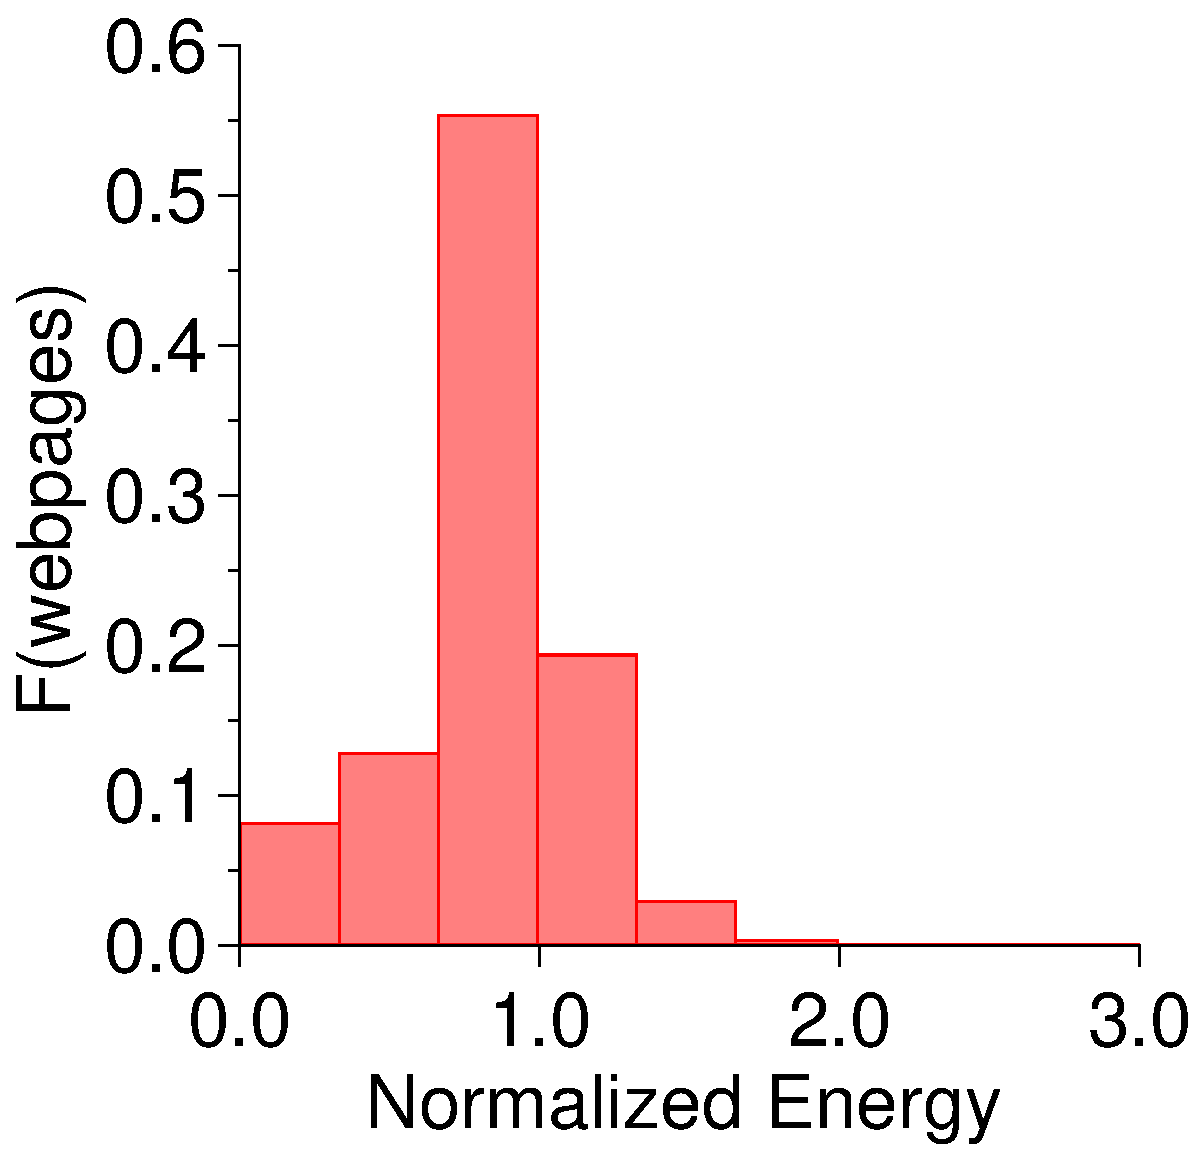
\includegraphics[trim=0 0 0 0, clip, width=.45\columnwidth]{webpage-aware}
\label{fig:webpage-aware}
}
\hspace*{15pt}
\subfloat[Relative energy of the integrated scheduler against the webpage-aware scheduler.]{
  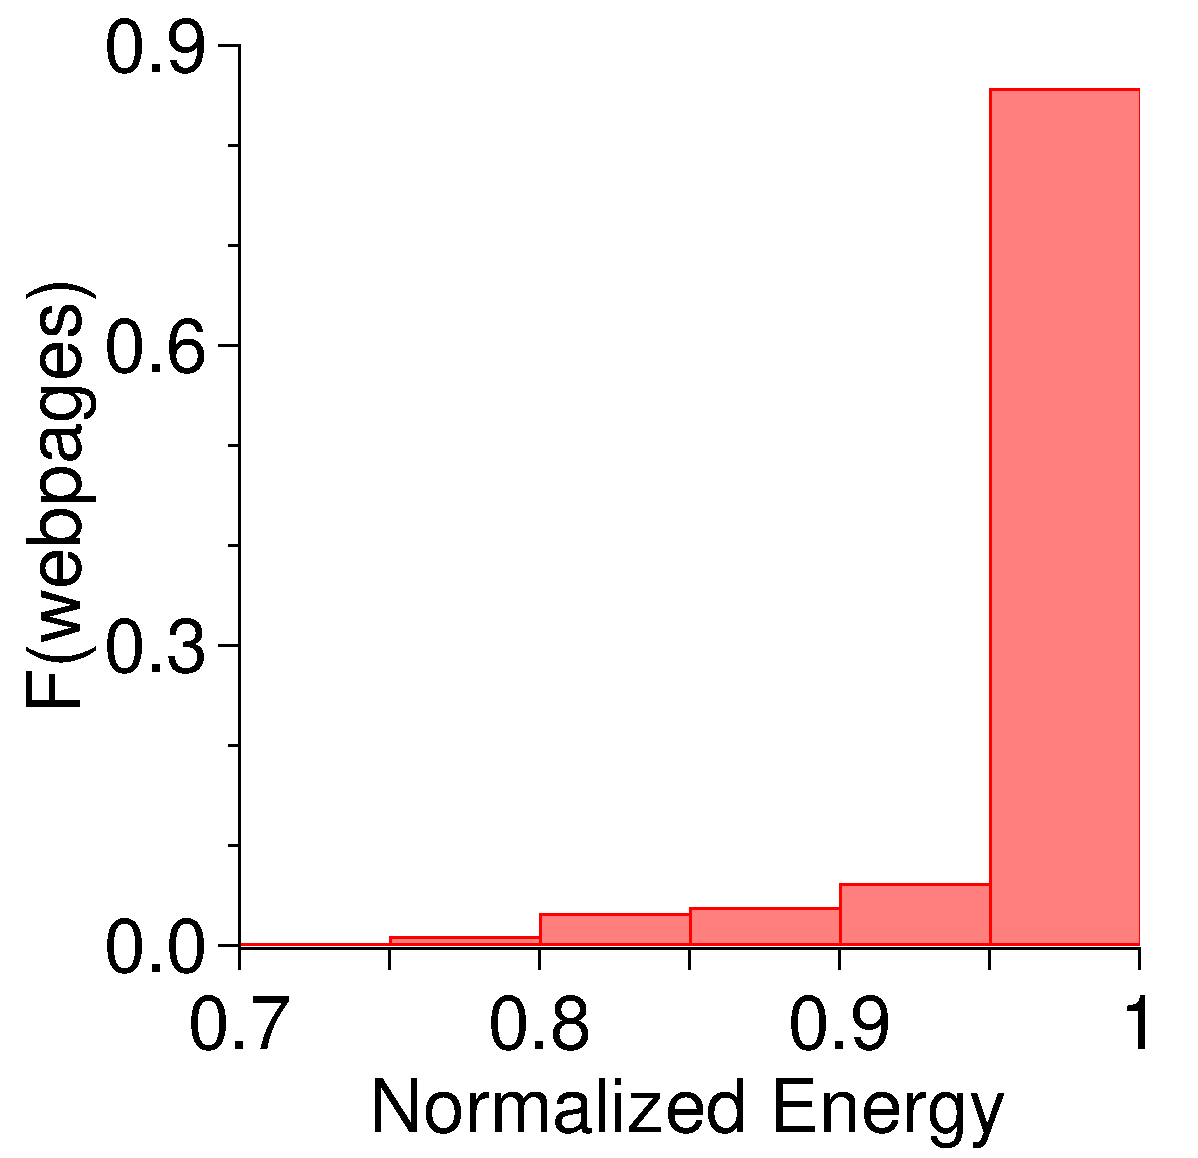
\includegraphics[trim=0 0 0 0, clip, width=.45\columnwidth]{integrated}
\label{fig:integrated}
} 
\caption{Distribution of per-webpage energy comparisons.}
\label{fig:e_saving}
\end{figure}

Specifically, the webpage-aware scheduler first restricts the OS DVFS scheduling space to two frequencies: a lower frequency that just meets the cut-off constraint and a upper frequency that just misses the constraint. Given the two frequencies, the webpage-aware scheduler tries to ensure that the cut-off latency can still be met by further tuning the percentage of time spent in either frequency. In practice, we set the \textsf{scaling\_max\_freq} and \textsf{scaling\_min\_freq} of the Linux cpufreq-governor to the lower and upper frequency, respectively. We set the \textsf{up\_threshold} to control when to promote to the higher frequency~\cite{ondemand}. For example, for \website{www.autoblog.com} (top-left in~\Fig{fig:pareto}), the OS DVFS on the big core would only operate on 1.2~GHz and 920~MHz. Because 920~MHz is nearly able to hit the deadline, only a small portion of the webpage load must be run in the upper frequency.  

\Fig{fig:integrated} shows, under a 3 seconds cut-off constraints, the histogram of per webpage relative energy of the integrated scheduler to the webpage-aware scheduler.  The integrated scheduler consistently out-performs the webpage-aware scheduler with 3.0\% average energy savings (up to 30\%).  We leave the full integration and detailed comparison for future work.

\section{Event-based Scheduling}
\label{sec:runtime:ebs}

I propose event-based scheduling (EBS) as the mechanism to optimize energy-efficiency for the Touching (T) and Moving (M) interactions. Each T or M interaction is internally translated to an application event. EBS is based on the observation that a T or M event may occur repetitively throughout a Web application usage session such that it is possible to predict the ideal architecture configuration of an event based on its history information of performance and energy consumption. We first present our motivation for performing event-based scheduling at the event handler level (\Sect{sec:runtime:ebs:char}). We then provide a high-level design overview of the event-based scheduling framework~(\Sect{sec:runtime:ebs:overview}) and then describe its implementation details~(\Sect{sec:runtime:ebs:sched}).

\subsection{Scheduling Unit}
\label{sec:runtime:ebs:char}

The scheduling unit in the event-based scheduler is the event handler. Whenever an event is triggered, a corresponding event handler is executed. \Fig{fig:runtime} provides an example, showing how event handlers H1, H2, and H3 (in that order) are pushed into the event queue for execution. For events that share the same performance constriant, we find that their event handlers have different execution latencies, and therefore lead to different performance slacks. We must treat each event handler differently and make scheduling decisions at that granularity.

We explain the variation in the event handlers' execution behavior using the Ember.js-based todo list application. \Fig{fig:slack} shows the sorted execution latencies of all the event handlers. The $x$-axis corresponds to the event handlers and the $y$-axis corresponds to the event handlers' execution latencies. In this example, we assume that the performance target for the scheduler is 100~ms, which is a common performance target for a smooth responsiveness.

\begin{figure}[t]
\centering
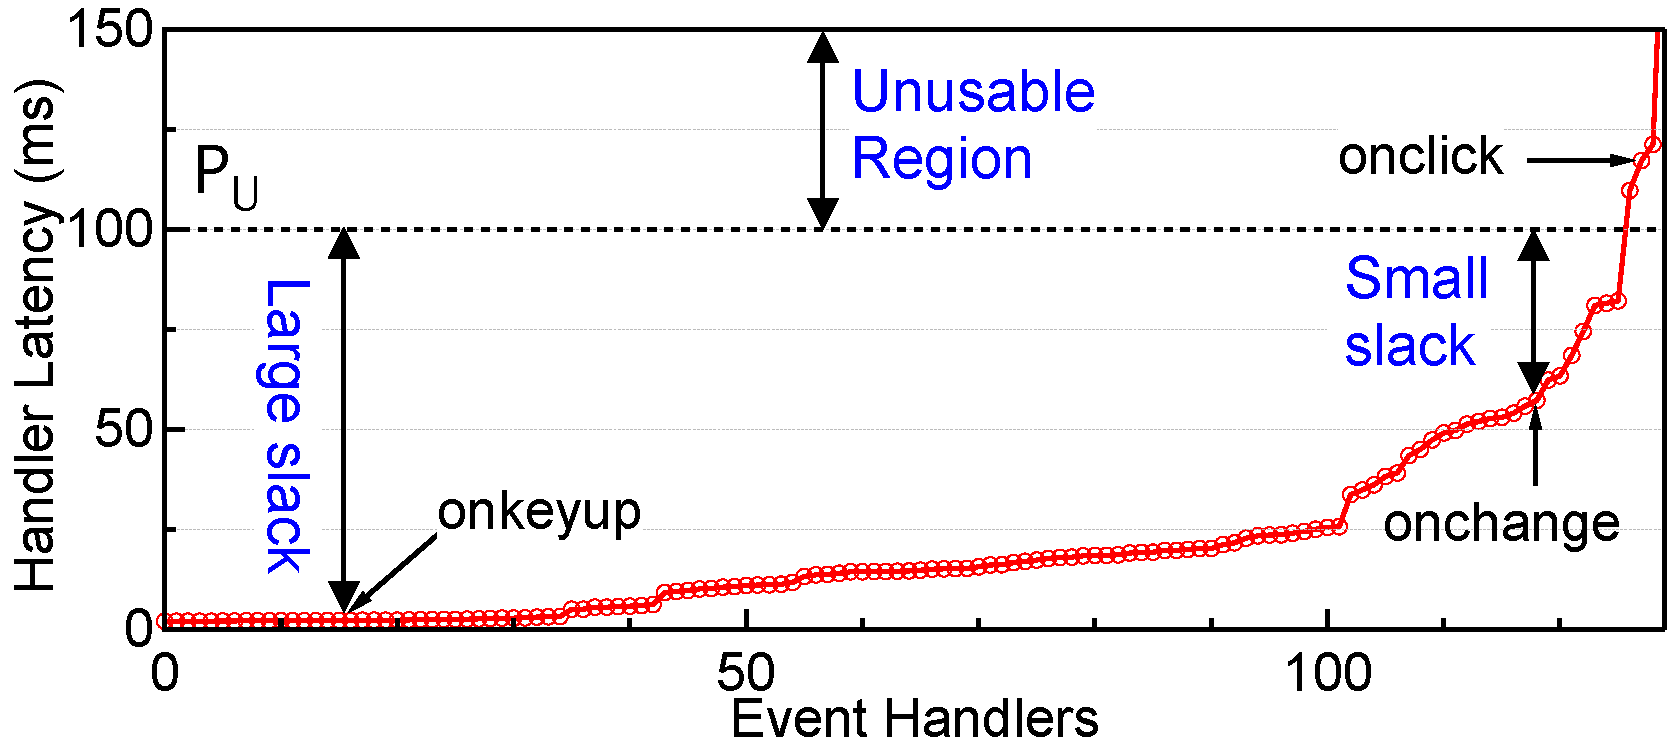
\includegraphics[trim=0 0 0 0, clip, width=0.9\columnwidth]{slack}
\caption{Event handler variation in Ember.js todo list application.}
\label{fig:slack}
\end{figure}

We observe a large latency variation for the handlers in~\Fig{fig:slack}. We label three of the application's representative event handlers as the application executes: \texttt{onkeyup},~\texttt{onchange}, and~\texttt{onclick}. The~\texttt{keyup} event handler only processes one keystroke and therefore finishes execution very quickly in just 2~ms, which leaves a large amount of slack (98\%) for the scheduler to exploit. In contrast, the~\texttt{onchange} event handler adds one entry into the todo list. It requires about 50~ms for execution, which translates to only about 50\% slack in performance. Lastly, the~\texttt{onclick} event handler deletes all the entries in the todo list. The processing time exceeds the performance constraint, and as such there is no opportunity to exploit performance slack. Instead, it requires a higher performance configuration, if available.

\subsection{Scheduler Design Overview}
\label{sec:runtime:ebs:overview}

\begin{figure*}[t]
\centering
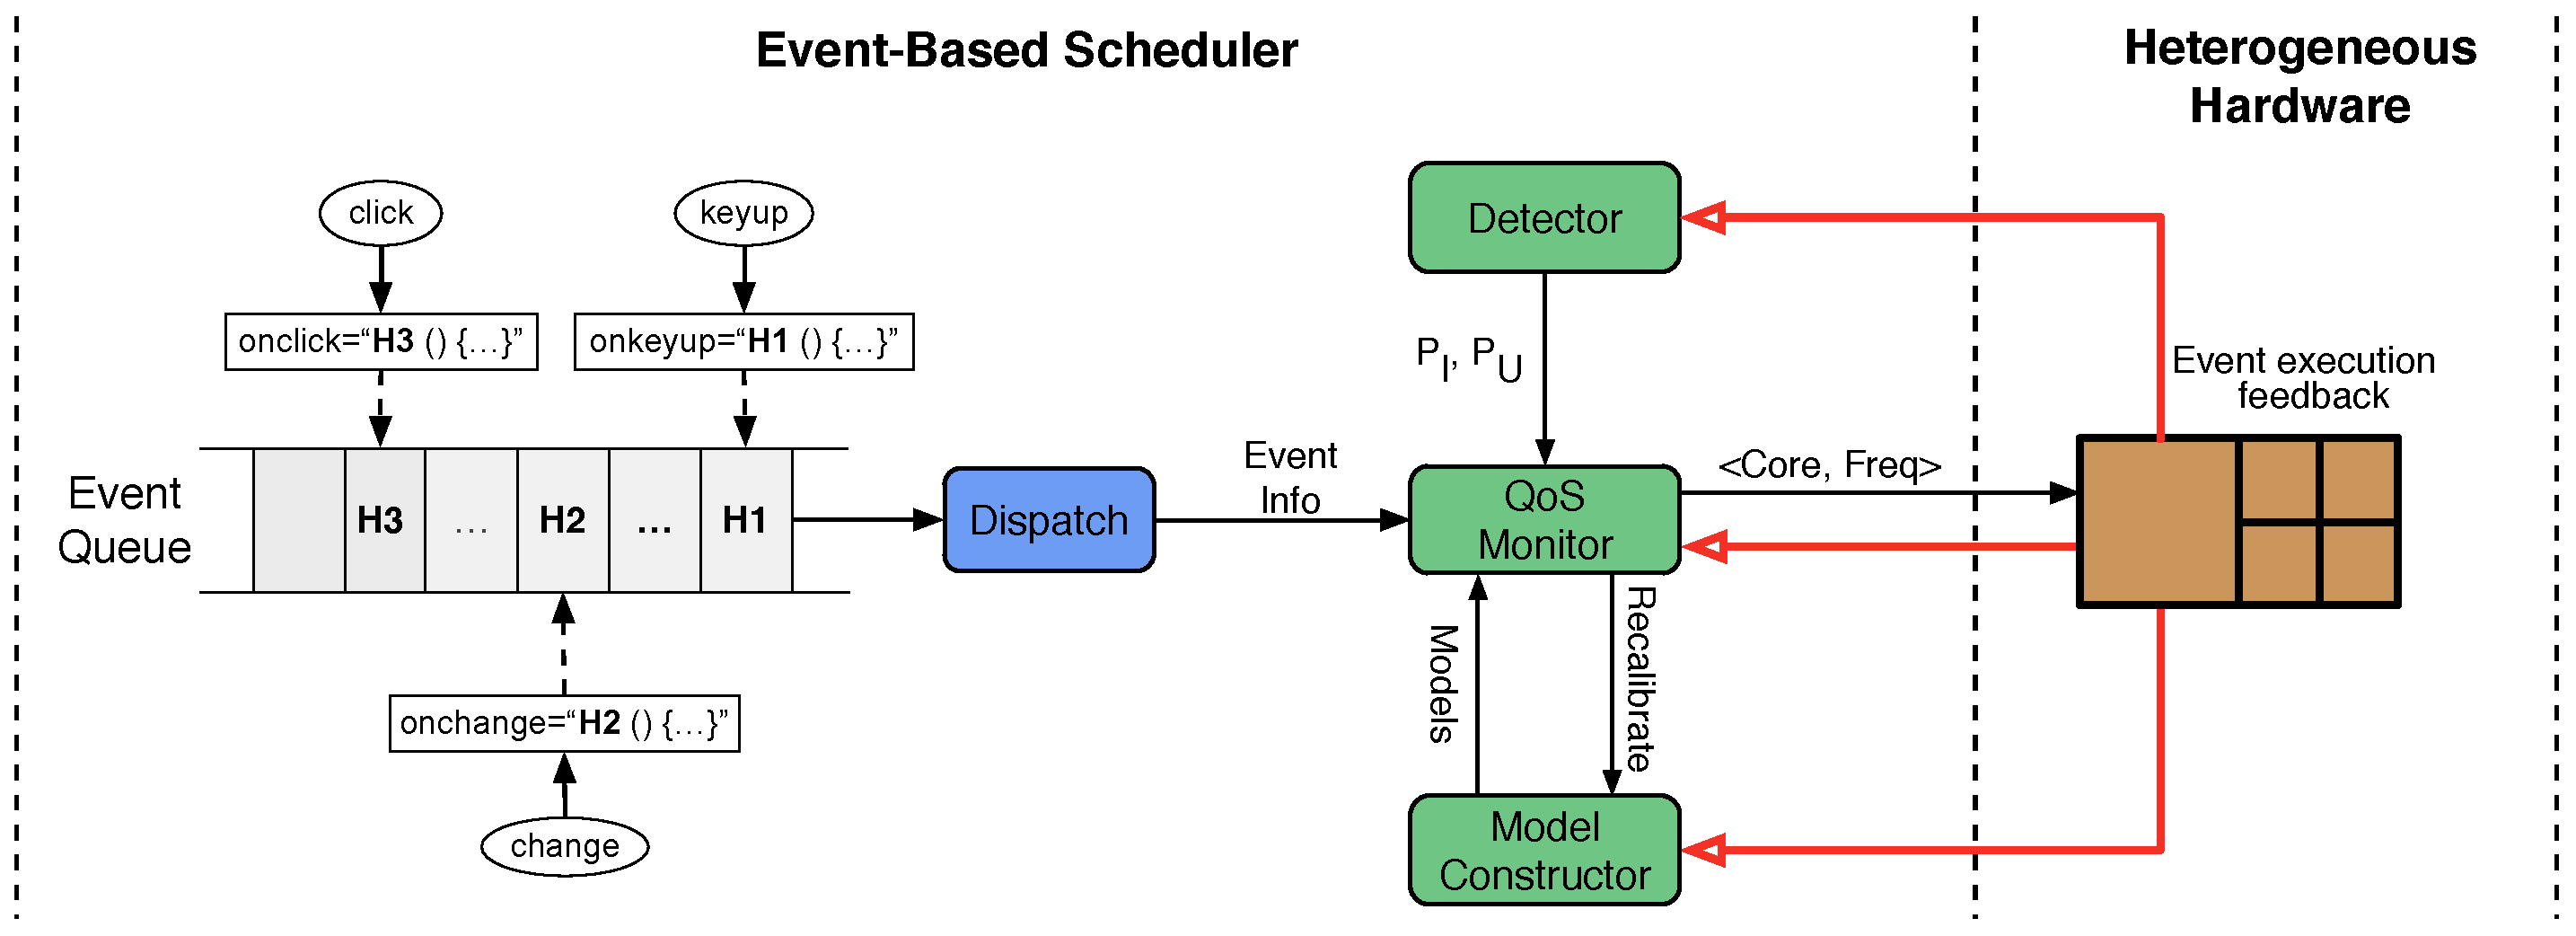
\includegraphics[trim=0 0 0 0, clip, width=\columnwidth]{runtime}
\caption{Event-based runtime scheduling framework.}
\label{fig:runtime}
\end{figure*}
\label{sec:runtime:overview}

The event-based scheduler predicts the ideal heterogeneous architecture execution configuration (i.e., a $\langle core, frequency \rangle$ tuple) whenever an event is triggered and the corresponding event handler is executed such that it ``barely'' meets the performance target with minimal energy consumption. It is important to emphasize that one event may lead to multiple frames being updated. Therefore, the \greenweb runtime operates on a per-frame basis as frames are what ultimately dictate user perceivable experience. If an event execution only produces one frame, the runtime finds the ideal execution configuration for the single frame associated with the event. If an event's execution leads to a sequence of frames such as in an animation, the runtime continuously identifies the ideal execution configuration for each frame until all the frames associated with the event are produced. All the associated frames share the same QoS target of the event.

The key idea of identifying an event's ideal execution configuration is to build a performance model and an energy model. They predict an event's latency and energy consumption under any core and frequency combination. With the two models, EBS sweeps all possible core and frequency combinations and selects the one that meets the QoS target with minimal energy.

The scheduler consists of a simple dispatch frontend and scheduling backend as illustrated in~\Fig{fig:runtime}. The frontend \textit{Dispatch} unit extracts relevant event information, and passes it to the backend. The backend consists of a \textit{Detector}, a \textit{Model Constructor} and a \textit{QoS Monitor}. The detector automatically identifies each event's QoS requirement. In its simplest form, the detector assumes a default latency target, such as 100~ms, for each event. If an event is annotated with programmer-guided QoS hints such as those enabled by the \greenweb language extensions as I will discuss in \Sect{sec:lang}, the detector can also extract the specified QoS information from the application. The model constructor builds a performance and energy model for each event. The models and event QoS information are then fed into the QoS monitor, which predicts the architecture configuration for executing an event while meeting the specified QoS target.

During application execution, the QoS monitor keeps monitoring event execution time and energy consumption on the hardware and uses the information to adjust its prediction and scheduling decisions on the fly, similar to conventional feedback-driven optimizations~\cite{FDO}. We will explain the detailed operation of the monitor in the next subsection. Intuitively, it is possible for the performance and energy models to underpredict or overpredict the architecture configuration. Under such circumstances, the monitor can decide to tune the predicted frequency or transition between big and little cores. If the models are deemed completely unusable, the monitor informs the model constructor to recalibrate the models. We now describe some key implementation details of the QoS monitor operations.

\subsection{Scheduler Implementation Details}
\label{sec:runtime:ebs:sched}

\paragraph{Performance Model} We construct performance models for big and little cores separately. Each model predicts the event handler execution latency under different frequencies. We use the classical DVFS analytical model initially proposed in~\cite{dvfs_model}, and employed in subsequent work, such as~\cite{dvfs_power}:
\begin{align*}
Execution\,\,\,time = T_{memory} + N_{dependent}/f
\end{align*}
where $f$ is the CPU frequency, $T_{memory}$ is the absolute memory access time that does not change with respect to the CPU frequency, and $N_{dependent}$ is the number of CPU cycles that are not overlapped with the memory accesses.

Strictly speaking, $N_{dependent}$ is a function of $f$. However, precisely constructing a model that varies $N_{dependent}$ with $f$ is complex and introduces a large calibration overhead at runtime. In our experiments, we find that it is feasible and necessary to trade model precision for performance. In particular, we find that treating $N_{dependent}$ as a constant is sufficient in our case.

Given this simplification, the model constructor builds the model with the event latency under two different frequencies by calculating the value of $T_{memory}$ and $N_{dependent}$. The trade-off in choosing the two frequencies is that on one hand using two sufficiently different frequencies provides higher accuracy, since the execution latencies from closer frequencies are more susceptible to measurement noise. But on the other hand, using two frequencies that are extremely high and low may result in execution falling in the  imperceptible or unusable QoS regions, ultimately wasting energy. In our current implementation, we use the highest and the second-highest frequencies to construct the performance model. We find that the run-to-run variation for the data collected using these two frequencies is low, resulting in a robust model.

\begin{figure}[t]
  \centering
  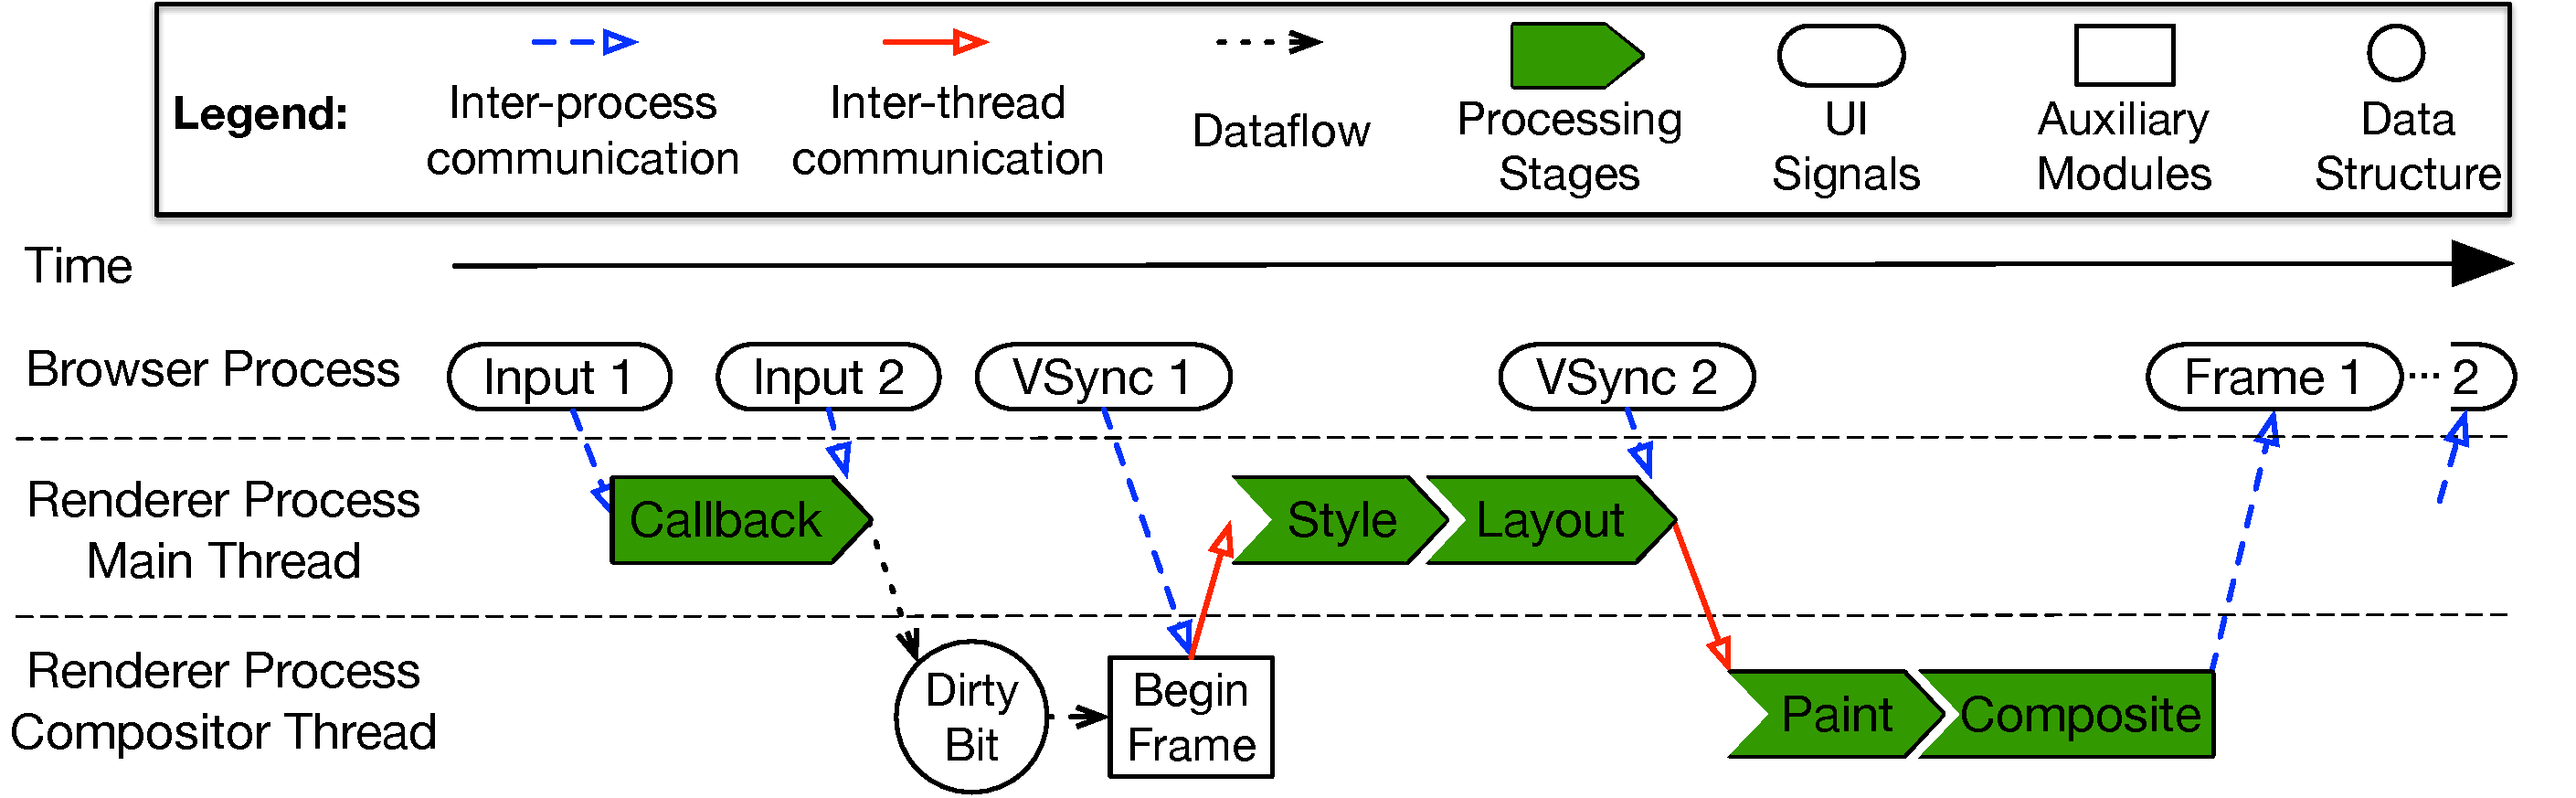
\includegraphics[trim=0 0 0 0, clip, width=\columnwidth]{inputs}
  \caption{The simplified view of frame lifetime in modern multiprocess/thread browsers. A frame starts when the browser process receives an input event and ends when the frame is displayed and the browser process is signaled. In between, an input event is processed by different stages spread across multiple threads. Different input events might interleave with each other.}
  \label{fig:inputs}
\end{figure}

\paragraph{Frame Latency Tracking} Tracking frame latency is crucial to constructing the performance and energy model. However, accurate frame latency tracking is a nontrivial task, primarily because of the complexities involved in generating a frame in modern Web browsers. Most prior work either is concerned only with the callback latency~\cite{ebs,efetch}, which, as we will show later, contributes to only a portion of frame latency, or it considers logical latency (e.g., the number of conditionals evaluated), which is insufficient to construct the prediction models~\cite{eventbreak}.

Accurately tracking frame latency requires us to understand how a frame is processed internally by a Web browser. Using Google Chrome browser as an example, \Fig{fig:inputs} illustrates a typical frame lifetime, starting from when an input event is received by the browser to when the frame is generated. Although we focus on Chrome, the execution model is generally applicable to almost all modern Web browsers such as Firefox, Safari, Opera, and Internet Explorer.

The browser process receives an input event and sends it to the renderer process, which applies five processing stages to produce a frame: callback execution, style resolution, layout, paint, and composite~\cite{renderingpipeline}. In the end, the browser process receives a signal indicating that the frame is produced. To improve performance, the processing stages are spread across two threads, and some portion of the composite stage could be offloaded to GPU (not shown). Note that our performance model in \Equ{eq:dvfs} captures the GPU processing time.

The key to latency tracking is to accurately attribute a frame to its triggering input. Two complexities of the frame generation process make frame attribution non-trivial. First, different input events might be interleaved. For the example in \Fig{fig:inputs}, Input 2 is triggered before Input 1 finishes. Naively associating an input event with its immediate next frame in this case would mistakenly attribute Frame 1 to Input 2.

Second, one frame might be associated with multiple input events. This is because modern browsers generate a new frame only when the display refreshes, i.e., a VSync signal arrives (typically 60~Hz on a mobile device), to avoid screen tearing~\cite{jankbusting,vsync}. If multiple callback functions have been executed before a VSync arrives, their effects are batched and cause only one frame. The batching is achieved through a \textit{dirty bit}. Each callback sets a dirty bit to indicate whether a new frame is needed as a result of callback execution. Callbacks from different inputs write to the same bit, but as long as one callback sets the dirty bit, a new frame will be generated when the browser later receives a VSync signal.

\begin{figure}[t]
  \centering
  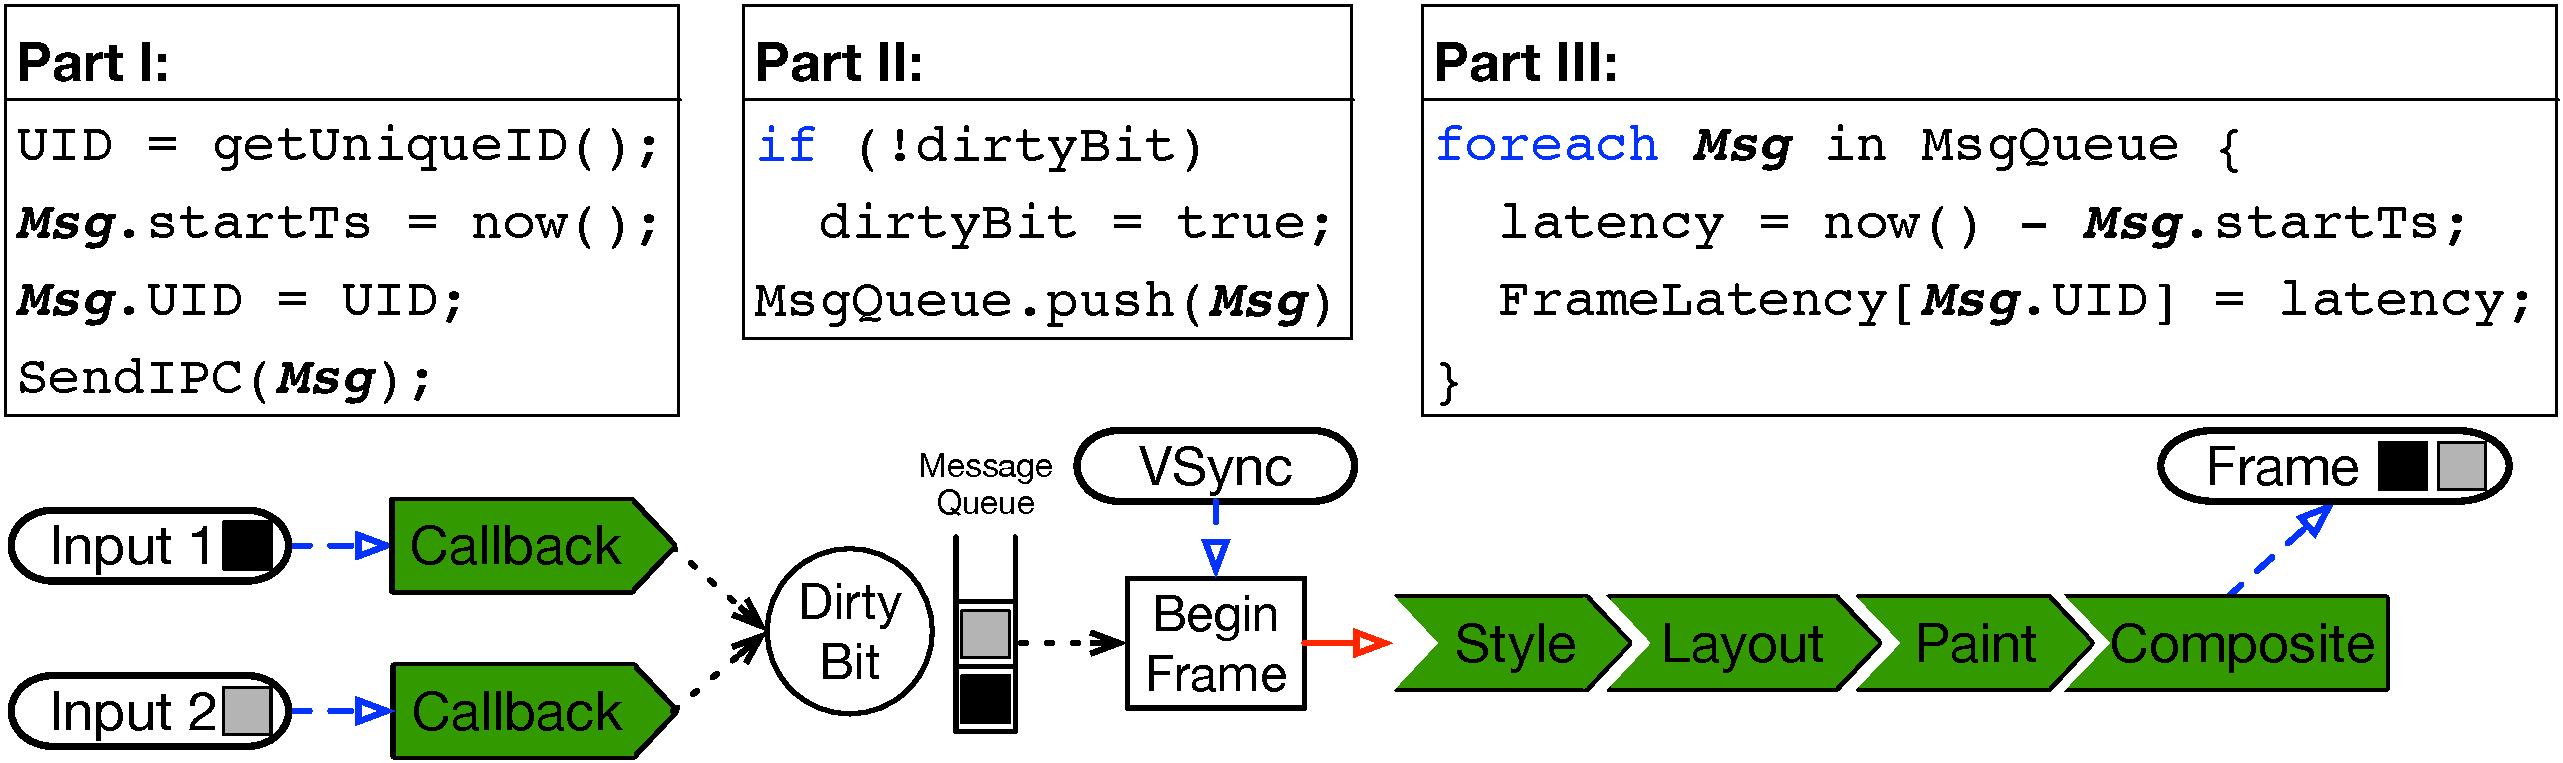
\includegraphics[trim=0 0 0 0, clip, width=\columnwidth]{tracking}
  \caption{Frame tracking algorithm. The key idea is to attach each input event with a metadata (\texttt{Msg} in the code) that uniquely identifies an input event and is propagated with the event. We use two colors to represent metadata of two different events in this example.}
  \label{fig:tracking}
\end{figure}

We show the flow of our tracking algorithm in \Fig{fig:tracking}. The key idea is to attach each input event with a piece of metadata (\texttt{Msg} in the code) that is propagated with the event throughout the entire processing pipeline. Each \texttt{Msg} is assigned with an ID that uniquely identifies an input (Part \RNum{1}). To track batched input events, the dirty bit system is augmented with a message queue, which stores \texttt{Msg} metadata of all input events that access the dirty bit after the previous VSync. All messages in the queue get propagated when the VSync signal arrives (Part \RNum{2}). When the browser receives the frame ready signal, it iterates through all the messages propagated with the signal and calculates the frame latency of each input based on their unique ID (Part \RNum{3}).

\paragraph{Energy Model} The energy model predicts the energy consumption of an event handler's execution. We construct the energy model on the basis of the performance model and the estimated power consumption. We derive the power estimation of all the core and frequency combinations by performing a profiling run and storing the results in a local power profile file that is read by the Web browser upon every launch. Persistently storing and looking up the power profile file aligns with the Android standard~\cite{powerxml}. Alternatively, we can dynamically derive the power consumption if power proxy counters, such as Running Application Power Limit (RAPL)~\cite{rapl}, are available and exposed to software. In our case, a rough estimate of the power consumption is sufficient.

\paragraph{QoS Monitor's Operation} The monitor uses deterministic finite automation (DFA) for each event handler to keep track of what architectural configuration it needs to provide for the event handler's execution. The first two times an event handler is executed, the QoS monitor informs the model constructor to build the performance and energy models. This lets the monitor predict the architecture configuration during all subsequent executions of the event handler.

After the initial model construction, the QoS monitor keeps monitoring the event handler's execution in order to perform fine-grained tuning. More specifically, the monitor compares the measured event handler execution latency with the scheduling target. The monitor conservatively deems the event handler's model as overpredicting (or underpredicting) if the measured value is lower than 80\% (or higher than 90\%) of the target latency. We empirically adopt these two threshold values because they are found to be effective in practice. Using a two-bit saturating counter, the monitor then increases the frequency by 100~MHz or transitions from the little core to the big core if model is underpredicting, or vice versa.

The monitor switches from fine-tuning an event handler's execution to recalibrating its model if it detects that the model is not performing well. We use a simple heuristic that is efficient in practice. If the model mispredicts (i.e., either underpredicts or overpredicts) more than four consecutive times, the monitor requests the model constructor to recalibrate.

\paragraph{Overheads} The QoS monitor accounts for scheduling overheads, which consist of two components: the overhead of the scheduling algorithm itself and the overhead of changing the architecture configuration (i.e, big/little core migration and/or frequency scaling). The scheduling algorithm's overhead is dominated by model construction, which only requires solving a two-variable linear system that imposes almost negligible overhead. For changing the architecture's configuration, we assume 100~$\mu$s for frequency scaling and 20~$\mu$s for switching cores, as indicated in~\cite{arm-bl-sw-wp,arm-bl-wp}.

\subsection{Experimental Setup}
\label{sec:runtime:ebs:setup}

\paragraph{Software Infrastructure} We implement \greenweb and its runtime system in Google's open-source Chromium browser engine, which is used directly in the Chrome browser and is the core of many other popular browsers, such as Opera and Android's default browser. Our implementation is based on Chromium version 48.0.2549.0, which is the most recent version at the time of our work. The modified Chromium runs on unmodified Android version 4.2.2.

\paragraph{Hardware Platform} We use the ODroid XU+E development board~\cite{odroidxue}, which contains an Exynos 5410 SoC that is known for powering the Samsung Galaxy S4. The Exynos 5410 SoC contains a representative ACMP architecture comprising an energy-hungry high-performance (big) core cluster and an energy-conserving low-performance (little) core cluster. The big and little clusters can be individually disabled and enabled. The big cores are ARM Cortex-A15 processors that operate between 800~MHz and 1.8~GHz at a 100~MHz granularity. The little cores are ARM Cortex-A7 processors that operate between 350~MHz and 600~MHz at a 50~MHz granularity. The frequency switching and core migration overhead is \SI{100}{\mu\second} and 20~$\mu$s, respectively~\cite{big-little,ebs}.

\paragraph{Energy Measurement}  \greenweb focuses on the processor power consumption because the processor power has been steadily increasing and has gradually become the most significant power consumer in a mobile device compared to other components such as the screen and radio~\cite{mobilecpu}.

We measure the processor power and energy consumption on real hardware as follows. The ODroid XU+E development board has built-in current sense resistors (\SI{10}{\milli\ohm}) for both the big and little cores. We use a National Instrument DAQ Unit X-series 6366 to collect voltage measurements at these sense resistors for the big and small CPU clusters at a rate of 1,000 samples per second, and thereby derive the power consumption. Energy consumption is computed by multiplying power with real execution time (\textit{not} the estimated time from the timing prediction model).

\paragraph{Application Selection} \Tbl{tab:app} shows the applications we use for evaluation. We crawl them using HTTrack~\cite{httrack} and host them on our Web server to enable annotations (discussed later). We acknowledge that the network condition could be slightly better when accessing a local server. However, we believe it has minimal impact because many prior work has shown that computation dominates the performance and energy consumption for today's mobile Web applications~\cite{zhu2015role,huang2012close,big-little}. Overall, these applications cover a wide range of domains such as news, utility, etc., and are mostly among the top 200 websites as ranked by Alexa~\cite{alexa}.

\paragraph{Baseline} We compare \greenweb with two baselines:
\begin{itemize}
  \item \textit{Perf} is the policy that always runs the system at the peak performance, i.e., highest frequency in the big core in our setup. It is the standard policy for interactive applications to guarantee the best user QoS experience.
  
  \item \textit{Interactive} is Android's default \texttt{interactive} CPU governor designed specifically for interactive usages. It maximizes performance when the CPU recovers from the idle state, and then dynamically changes CPU performance as CPU utilization varies~\cite{android_cpufreq}.
\end{itemize}

\paragraph{Usage Scenarios} Real-world user study over one year span from the LiveLab project~\cite{livelab} shows that mobile users often have to interact with devices under different battery conditions. Therefore, we evaluate \greenweb under two primary usage scenarios based on battery status:
\begin{itemize}
  \item ``Imperceptible'' represents scenarios in which the battery budget is abundant, and users expect high QoS experience. It corresponds to the imperceptible QoS experience discussed in \Sect{sec:qos:target}. The imperceptible performance threshold $T_I$ is used as the QoS target.
  
  \item ``Usable'' represents scenarios in which the battery budget is tight and users could tolerate lower performance. It corresponds to the usable QoS experience. The usable performance threshold $T_U$ is used as the QoS target.
\end{itemize}

It is worth noting that \textit{Perf} and \textit{Interactive} behave the same independently of the usage scenario. \greenweb under these two scenarios is denoted by \textit{GreenWeb-I} and \textit{GreenWeb-U}, respectively, in the rest of the evaluation.

\paragraph{Reproducibility} We repeat every experiment that we study 3 times. Unless otherwise mentioned, the results we report are the median of all runs. We find the run-to-run variations are usually about 5\%, and do not affect our conclusions. We use Mosaic~\cite{mosaic}, a UI-level record and replay tool, to ensure consistent user interaction and to reduce human-induced noise across different runs on the same application.

% !TEX root = paper.tex

\begin{table}[t]
\Huge
\centering
\captionsetup{width=1\columnwidth}
\caption{\small List of applications. ``Time'' indicates full interaction duration. ``Annotation'' indicates percentage of events that are annotated. ``Events'' indicates the amount of events triggered during full interaction. Note: we only annotate and count events that are directly triggered by mobile user interactions as discussed in \Sect{sec:qos:interaction}. Applications marked with * are manually annotated because they are developed using libraries that \autogreen does not currently support. Their annotation percentage numbers are estimated.}
\renewcommand*{\arraystretch}{1.2}
\renewcommand*{\tabcolsep}{6pt}
\resizebox{1\columnwidth}{!}
{
%\begin{tabular}{l l | l c | c c l l}
%\toprule[0.15em]
%\bigstrut\textbf{Application} & \bigstrut\textbf{Domain} & \bigstrut\textbf{Interaction Description} & \bigstrut\textbf{\specialcell{Interaction\\Type (LTM)}} & \bigstrut\textbf{\specialcell{~~Lines\\of Code}} & \bigstrut\textbf{\specialcell{~~~Lines of\\Annotation}} & \bigstrut\textbf{QoS Type} & \bigstrut\textbf{\specialcell{QoS Target\\($T_I$, $T_U$)}}\\
%\midrule[0.05em]
%Amazon & Shopping & Horizontally swipe the Ads bar to see different Ads. & Moving & 4,300 & 4 & Continuous & (16.6, 33.3) ms\\
%BBC & News & Load the main webpage. & Loading & 1,734 & 4 & Single & (1, 10) s\\
%CamanJS & Utility & Tap a button to apply a complex image filter to a photo. & Tapping & 4,910 & 7 & Single & (1, 10) s\\
%Cnet & News & Tap a button to expand the main menu in animation. & Tapping & 3,687 & 4 & Continuous & (16.6, 33.3) ms\\
%Craigslist & Search & Scroll the page to find the ``outdoor'' category. & Moving & 800 & 5 & Continuous & (16.6, 33.3) ms\\
%Paper.js & Utility & Move finger to draw a series of curves. & Moving & 12,276 & 5 & Continuous & (16.6, 33.3) ms\\
%%http://146.6.28.88/paperjs/examples/Tools/Wave.html
%Goo & News & Tap news group title to switch to another group. & Tapping & 1,106 & 4 & Continuous & (16.6, 33.3) ms\\
%Google & Search & Load the main webpage. & Loading & 38 & 4 & Single & (1, 10) s\\
%MSN & News & Tap to display the menu bar. & Tapping & 1,941 & 6 & Single & (100, 300) ms\\
%Todo & Utility & Tap to delete all Todo List items. & Tapping & 238 & 6 & Single & (100, 300) ms\\
%UOL & News & Load the main webpage. & Loading & 25 & 6 & Single & (1, 10) s\\
%W3Schools & Education & Tap to show the sitemap. & Tapping & 1,382 & 3 & Continuous & (16.6, 33.3) ms\\
%Whatsapp & Utility & Tap to show the dropdown menu that swipes vertically. & Tapping & 273 & 6 & Continuous & (16.6, 33.3) ms\\
%Yahoo & News & Scroll the page to find football news. & Moving & 1,139 & 4 & Continuous & (16.6, 33.3) ms\\
%LZMA-JS & Utility & Tap the button to compress the jQuery library file. & Tapping & 3,297 & 8 & Single & (1, 10) s\\
%%http://www.html5rocks.com/en/tutorials/speed/txt-compression/#toc-txtfmt
%%For LZMA-JS, had to modify the original code logic because it uses a setImmediate to call the handler, which forces an additional frame.
%\bottomrule[0.15em]
  
\begin{tabular}{l | c l l | r r r}
\toprule[0.15em]
 & \multicolumn{3}{c}\bigstrut\textbf{Micro-benchmarking~~~~~~~~~~~~~~~} & \multicolumn{3}{|c}\bigstrut\textbf{Full Interaction~~~~~~~~~~}\\
\multirow{2}{*}\bigstrut\textbf{Application}  &  \bigstrut\textbf{Interaction} & \bigstrut\textbf{QoS Type}  & \bigstrut\textbf{QoS Target}  & \bigstrut\textbf{Time}  & \bigstrut\textbf{Events} & \bigstrut\textbf{Annotation}         \\
\midrule[0.05em]
BBC          & Loading   & Single        & (1, 10) s          & 0:86    & 60    &  20\%$^*$  \\
Google       & Loading   & Single        & (1, 10) s          & 0:31    & 26    & 87.5\%       \\
CamanJS      & Tapping   & Single        & (1, 10) s          & 0:49    & 24    & 100\%    \\
LZMA-JS      & Tapping   & Single        & (1, 10) s          & 0:53    & 39    & 100\%    \\
MSN          & Tapping   & Single        & (100, 300) ms      & 0:59    & 126   & 51.2\%    \\
Todo         & Tapping   & Single        & (100, 300) ms      & 0:26    & 26    & 38.3\%      \\
Amazon       & Moving    & Continuous    & (16.6, 33.3) ms    & 0:36    & 101   &   33\%$^*$  \\
Craigslist   & Moving    & Continuous    & (16.6, 33.3) ms    & 0:25    & 22    & 84.6\%      \\
Paper.js     & Moving    & Continuous    & (16.6, 33.3) ms    & 0:16    & 560    & 100\%   \\
Cnet         & Tapping   & Continuous    & (16.6, 33.3) ms    & 0:46    & 60    & 55.3\%   \\
Goo.ne.jp          & Tapping   & Continuous    & (16.6, 33.3) ms    & 0:16    & 23    & 51.8\%    \\
W3Schools    & Tapping   & Continuous    & (16.6, 33.3) ms    & 0:64    & 59    & 100\%    \\
\bottomrule[0.15em]
\end{tabular}
}
\label{tab:app}
%\vspace{-4pt}
\end{table}



\begin{figure}[t]
\centering
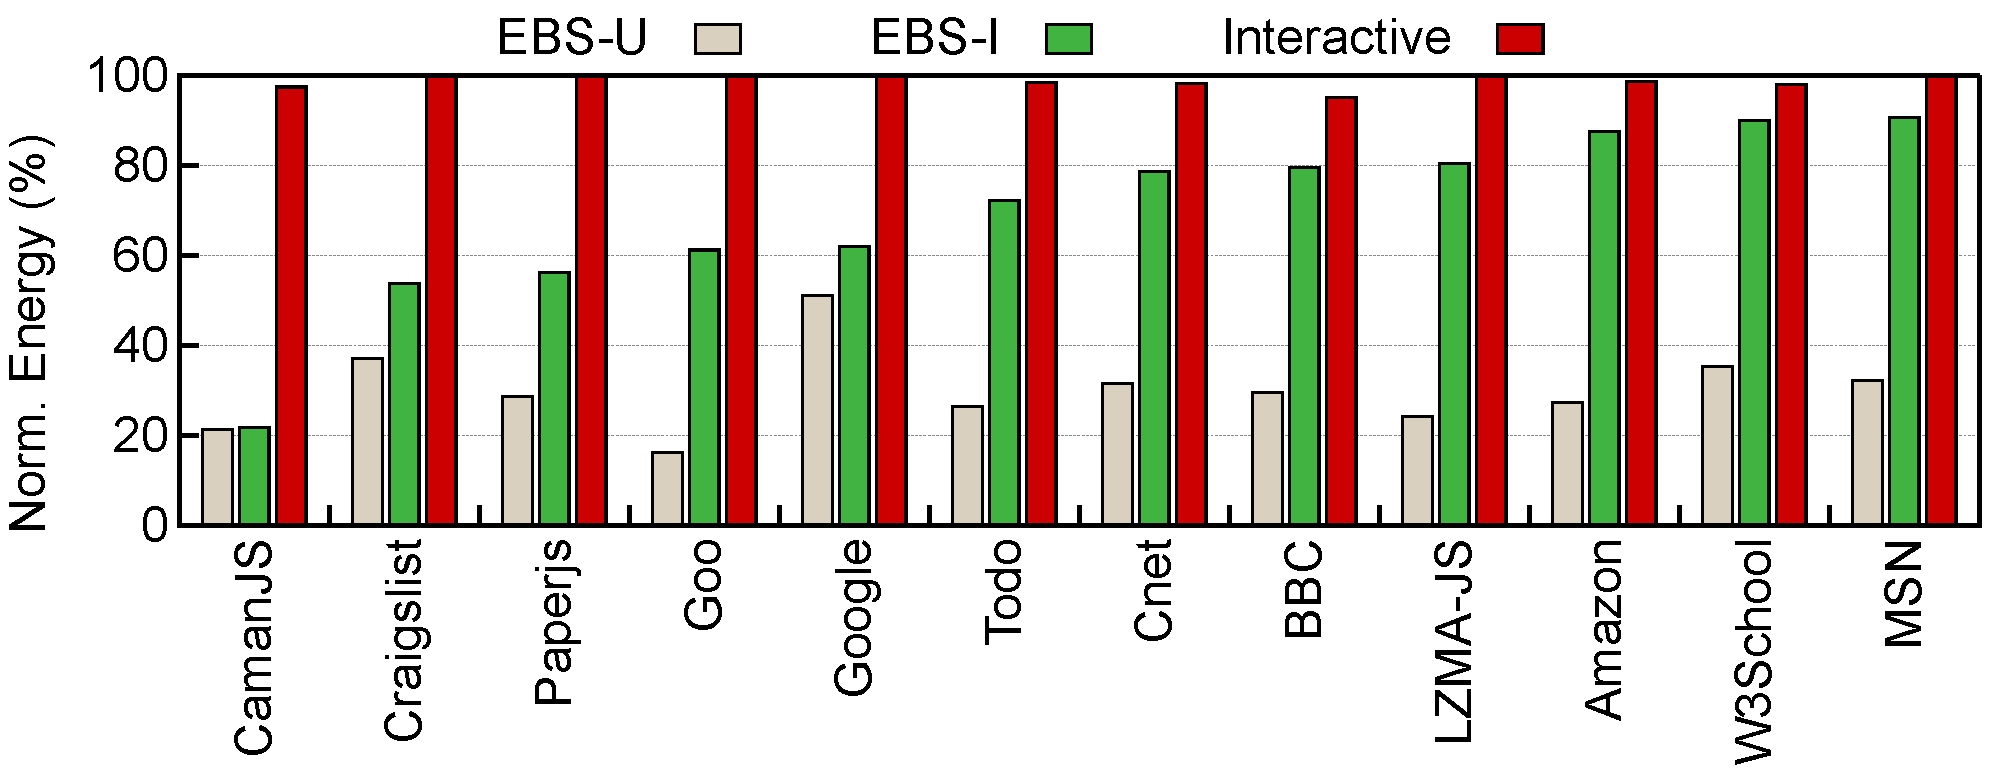
\includegraphics[trim=0 0 0 0, clip, width=\columnwidth]{energy_results_f}
\caption{Energy consumption normalized to \textit{Perf}. Lower is better.}
\label{fig:energy_results_f}
\end{figure}

\subsection{Evaluation}
\label{sec:runtime:ebs:eval}

\begin{figure}[t]
\centering
\subfloat[Architecture configuration distribution for \textit{GreenWeb-I}.]
{
        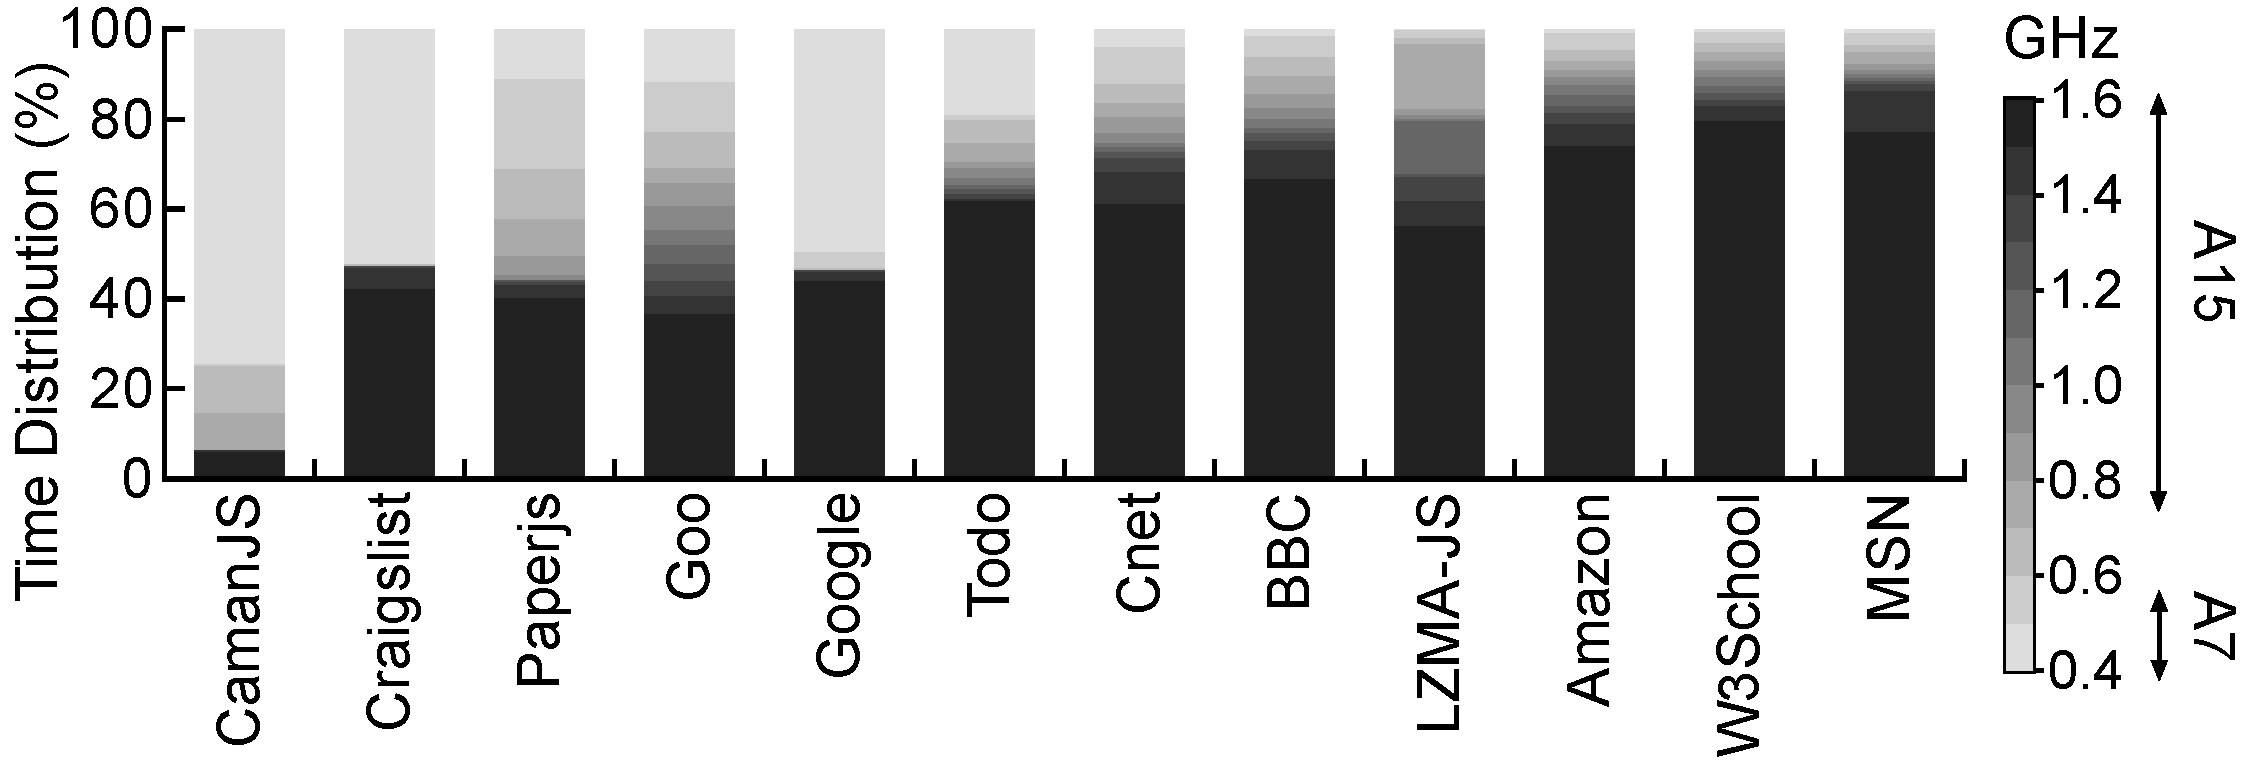
\includegraphics[trim=0 0 0 0, clip, width=1\columnwidth]{freq_dist_pi}
        \label{fig:freq_dist_pi}
}\\
\subfloat[Architecture configuration distribution for \textit{GreenWeb-U}.]
{
        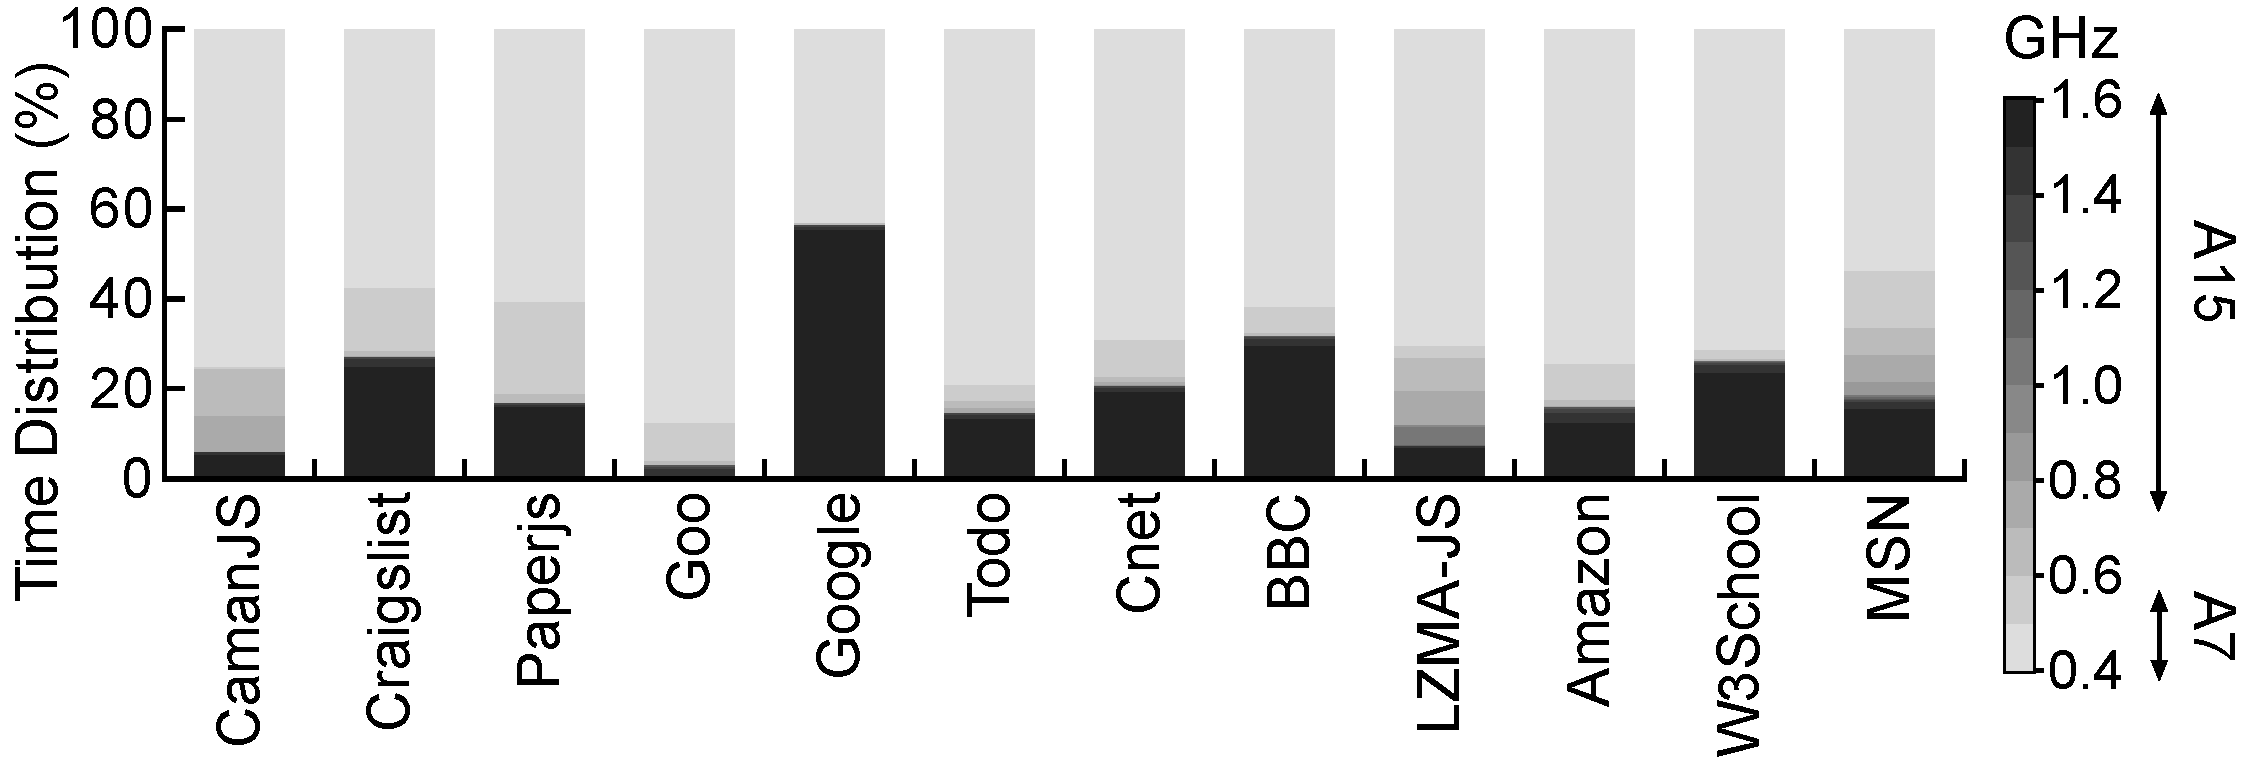
\includegraphics[trim=0 0 0 0, clip, width=1\columnwidth]{freq_dist_pu}
        \label{fig:freq_dist_pu}
}
\caption{The architecture configuration distribution under the ``imperceptible'' (\textit{GreenWeb-I}) and ``usable''  (\textit{GreenWeb-U}) usage scenario.}
\label{fig:freq_dist}
\end{figure}

In this section, we perform a sequence of interactions on each application, and evaluate the end-to-end behavior of \greenweb. Each sequence consists of a mix of LTM interactions and contains events with different QoS types and QoS targets. The ``Full Interaction'' category in \Tbl{tab:app} shows the details of each interaction. On average, each interaction sequence triggers about 94 events and lasts about 43~s.

We acknowledge that there are alternative ways to interact with each application. Thoroughly evaluating all the representative interactions with each application involves a large user study and is beyond the scope of this paper. However, we did perform our due diligence to make sure that the chosen interaction for each application is representative.

\paragraph{Energy Savings} \Fig{fig:energy_results_f} shows the energy consumption of \textit{Interactive} and \greenweb's two usage scenarios. The results are normalized to \textit{Perf}, and sorted in the ascending order of \textit{GreenWeb-I}. As compared to \textit{Interactive}, \greenweb achieves on average 29.2\% and 66.0\% energy saving under the imperceptible and usable usage scenarios, respectively.

\textit{Interactive} consumes energy close to \textit{Perf} across all applications, indicating that the Android \texttt{Interactive} governor is almost always operating at the peak performance. This is because user interactions, especially events with a ``continuous'' QoS type, typically generate a large volume of frames, which leads to high CPU utilization. \textit{Interactive} responds to the high CPU utilization by increasing CPU performance. With the QoS knowledge provided by developers, however, \greenweb can identify execution configurations that conserve energy while still meeting QoS requirements.

\paragraph{Architecture Configuration Distribution} To better understand the sources of energy savings of \greenweb, we examine the architecture configuration distribution of \greenweb under the imperceptible and usable usage scenario shown in \Fig{fig:freq_dist_pi} and \Fig{fig:freq_dist_pu}, respectively. Bars with darker colors indicate higher performance configurations.

We make two notable observations from the distribution results. First, \greenweb tends to bias toward big core (A15) configurations much more often under the imperceptible scenario (\Fig{fig:freq_dist_pi}) than under the usable scenario (\Fig{fig:freq_dist_pu}). This observation confirms the result that \textit{GreenWeb-I} has less energy saving than \textit{GreenWeb-U}. Second, the fact the \greenweb dynamically changes its execution configuration under different QoS targets indicates that the \greenweb can adapt to different user QoS expectations while saving energy. In contrast, \textit{Interactive} always adopts the same scheduling policy independent of the user QoS expectation, leading to energy waste. This observation indicates that an ACMP architecture is beneficial in mobile Web, but the burden is on the runtime system to intelligently leverage it.

\begin{figure}[t]
  \centering
  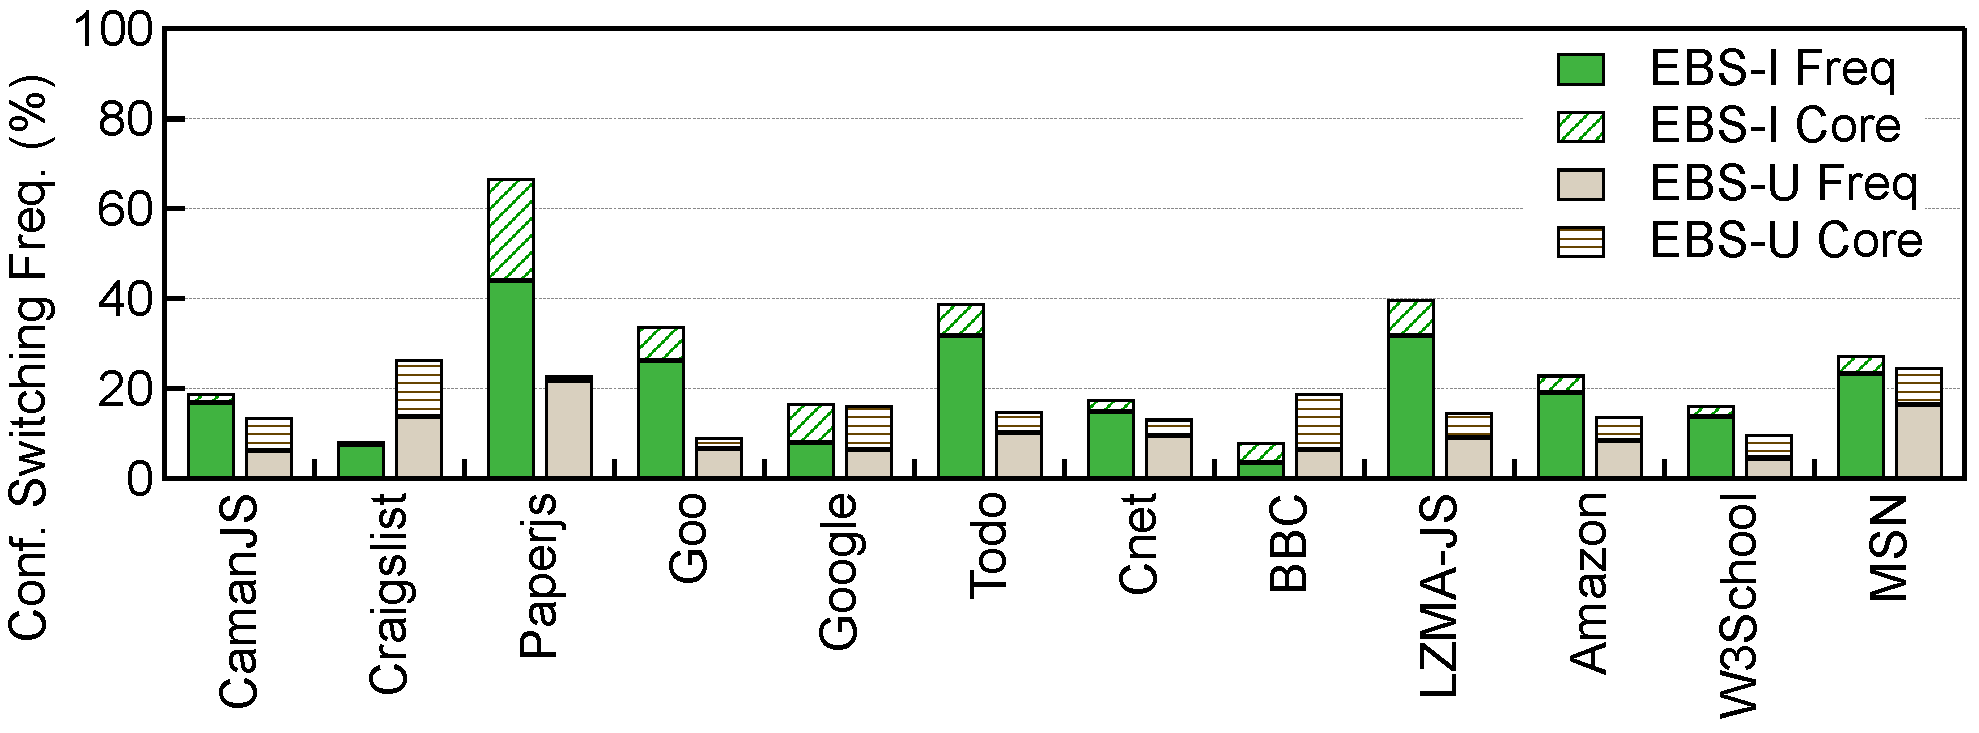
\includegraphics[trim=0 0 0 0, clip, width=\columnwidth]{freq_switch}
  \caption{Execution configuration switching frequency under \textit{GreenWeb-I} and \textit{GreenWeb-U}. Two configuration switching types exist: CPU frequency switch (solid) and core migrations (stripe).}
  \label{fig:freq_switch}
\end{figure}

\paragraph{Configuration Switching Frequency} Complementary to the distribution of architecture configuration, \Fig{fig:freq_switch} shows the switching frequency of architecture configuration in \textit{GreenWeb-I} and \textit{GreenWeb-U}. We decompose the configuration switching into two categories: CPU frequency change and core migration (between big and little clusters). Thus, \Fig{fig:freq_switch} is shown as a stacked bar plot where the frequencies of both categories are stacked for each application.

We draw three conclusions from the switching frequency statistics. First, \greenweb introduces only modest configuration switching (20\% on average). Recall from \Sect{sec:eval:setup} that the CPU frequency switching and core migration incur overhead only to the order of $\mu$s, much smaller than the QoS target which is typically to the order of millisecond. Therefore, the execution configuration has minimal performance impact.

Second, for most of applications \textit{GreenWeb-I} incurs more switchings than \textit{GreenWeb-U}. This is unsurprising because as compared to \textit{GreenWeb-U}, \textit{GreenWeb-I} optimizes for a tighter QoS target, which is more sensitive to frame (phase) variance and more vulnerable to frame performance mis-prediction. In contrast, a more relaxed QoS target is more robust against frame variance. Our results suggest that a better frame performance predictor such as the profiling-guided prediction~\cite{pgdvfs} would be helpful in reducing the execution configuration switching in the imperceptible mode.

Third, the CPU frequency change dwarfs core migrations and dominates the configuration switching. Thus, fast DVFS is desired. Our results suggest that a fast on-chip voltage regulator that is increasingly prevalent in server processors~\cite{fivr,ivr} is also beneficial in mobile CPUs.

\begin{figure}[t]
\centering
\subfloat[QoS violation comparison under the imperceptible usage scenario.]
{
        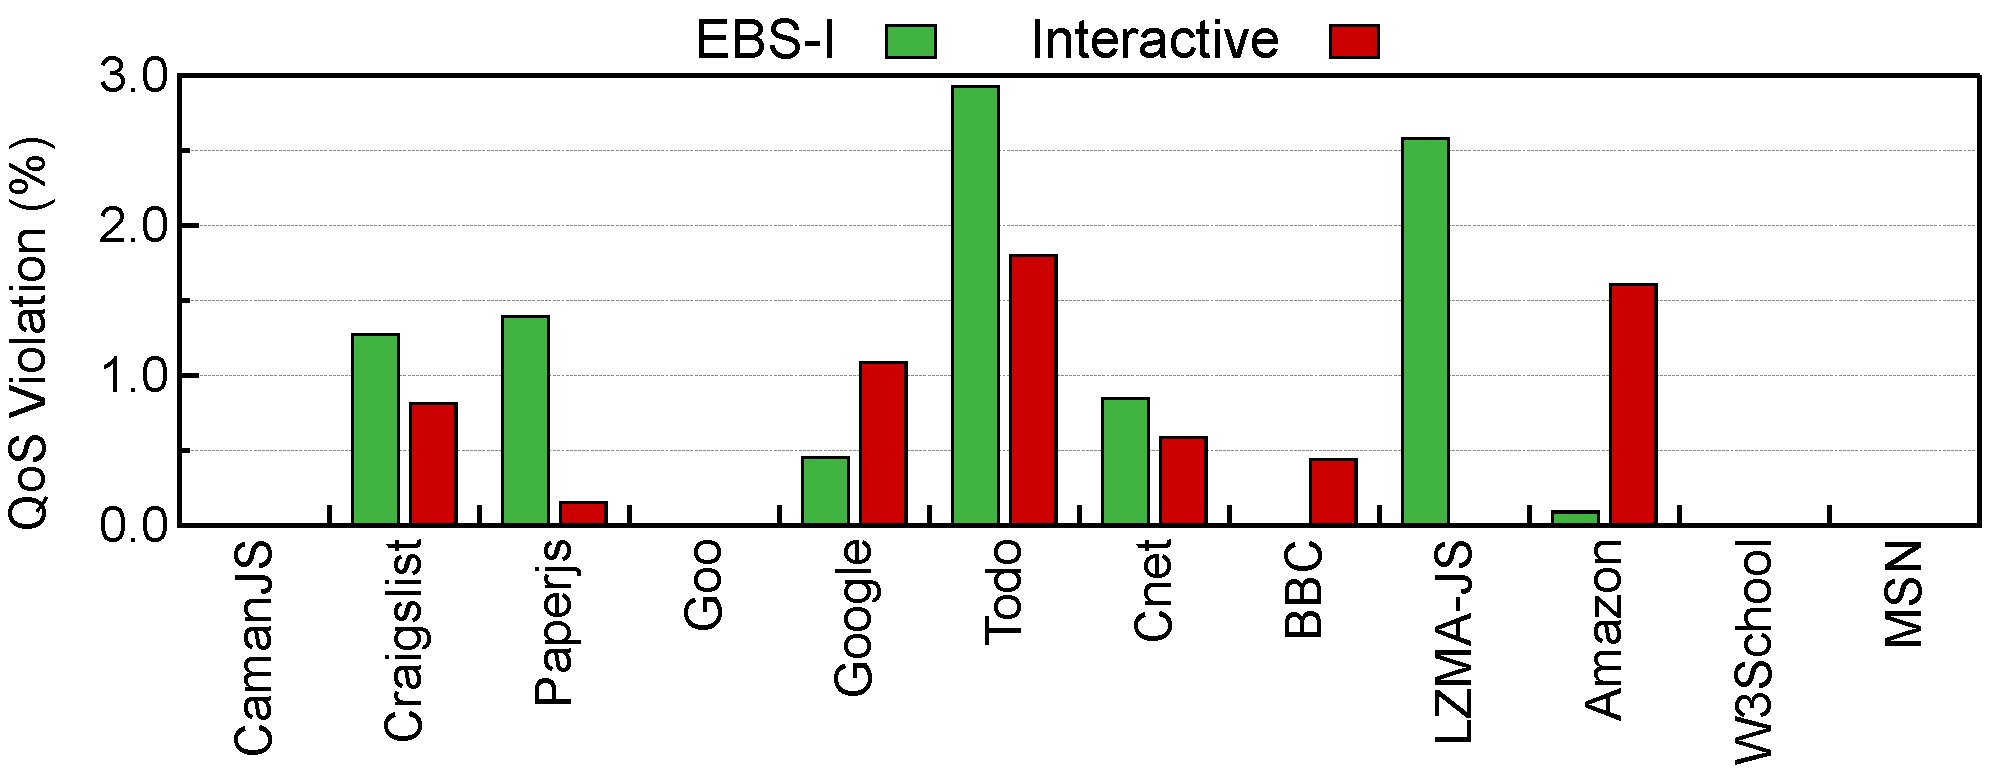
\includegraphics[trim=0 0 0 0, clip, width=.6\columnwidth]{qos_pi_results_f}
        \label{fig:qos_pi_results_f}
}\\
\subfloat[QoS violation comparison under the usable usage scenario.]
{
        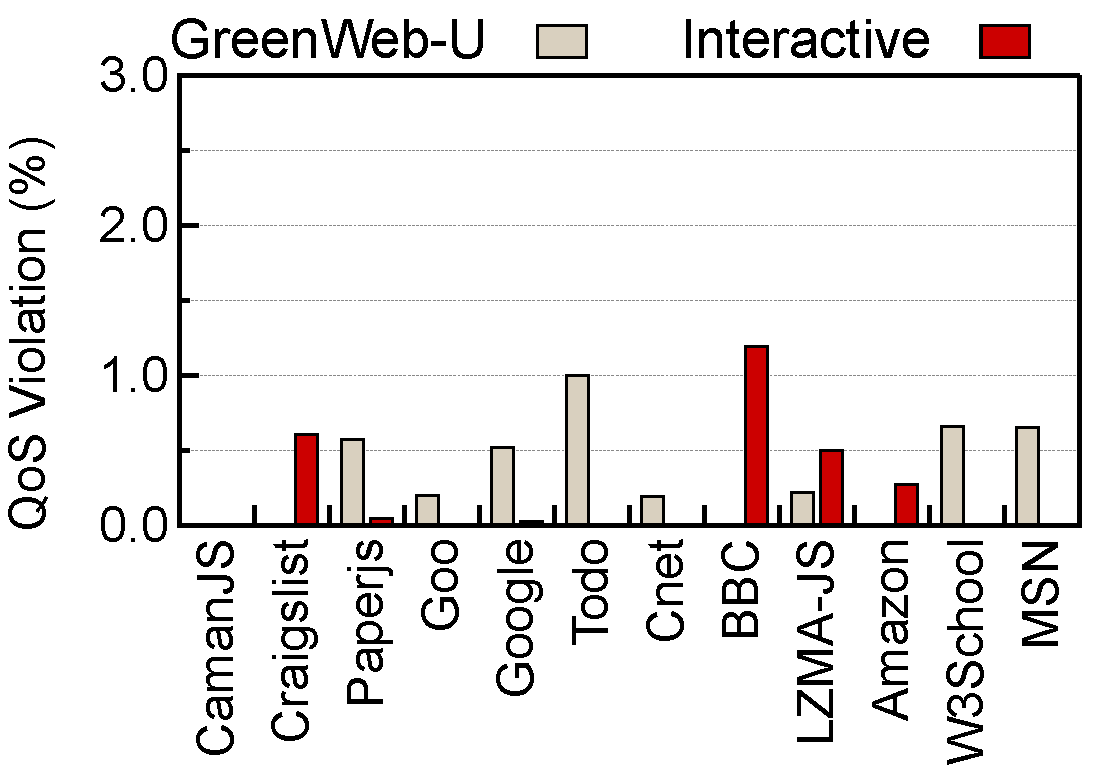
\includegraphics[trim=0 0 0 0, clip, width=.6\columnwidth]{qos_pu_results_f}
        \label{fig:qos_pu_results_f}
}
\caption{QoS violations are presented as additional violations on top of \textit{Perf}.}
\label{fig:full_results}
\end{figure}

\paragraph{QoS Violation} \Fig{fig:qos_pi_results_f} and \Fig{fig:qos_pu_results_f} show the QoS violation of \textit{Interactive} and \greenweb under the imperceptible and usable scenarios, respectively. On average, \greenweb introduces 0.8\% and 0.6\% more QoS violations than \textit{Perf} under the imperceptible and usable scenarios, respectively. The QoS violations are lower than in the microbenchmarks because the interaction duration gets longer and the QoS violations caused by profiling runs are amortized.

Compared to \textit{Interactive}, \greenweb has similar, in some cases fewer, QoS violations. Considering the significant energy savings, we conclude that the QoS-aware \greenweb system can use energy more wisely by being aware of user QoS expectations. Overall, \greenweb achieves better energy efficiency than the QoS-agnostic \textit{Interactive} scheme.

\section{Related Work}
\label{sec:runtime:related}

We first discuss prior scheduling work on ACMP because the particular implementation of \webrt presented in this work relies on the ACMP architecture (\Sect{sec:runtime:related:sched}). As the goal of \webrt is to save energy without sacrificing performance, we then discuss prior work on improving the performance (\Sect{sec:runtime:related:perf}) and energy consumption (\Sect{sec:runtime:related:energy}).

\subsection{Single ISA/DVFS Scheduling}
\label{sec:runtime:related:sched}

The particular implementation of \webrt is an example of utilizing single-ISA heterogeneous systems capable of DVFS for trading off performance with energy~\cite{single-ISA}. Nvidia's Kal-El~\cite{Tegra3} is a single-ISA heterogeneous system that integrates four high-frequency cores with one low-frequency core. ARM's proposed big.LITTLE system~\cite{big.little} contains an out-of-order Cortex-A15 processor and an in-order Cortex-A7 processor. ACMP architecture is already widely adopted in today's mobile SoCs shipped by major vendors such as Samsung and Qualcomm~\cite{exynos5biglittle}. We expect our \webrt implementation to be readily applicable to commodity mobile hardware.

The scheduling mechanism in \webrt differs from existing single-ISA scheduling and DVFS techniques in three key aspects: scheduling \textit{unit}, scheduling \textit{objective}, and scheduling \textit{heuristics}. First, the scheduling unit in existing techniques is either interval based (fixed-instruction interval~\cite{single-ISA,compositecores,tracephase,tm,DVFSPred} or fixed-time interval~\cite{DCS,MIPJ,PIE,ondemand,unfairsched}) or a code segment (e.g., critical sections, lagging threads, application kernels~\cite{acs,bis,uba,YinYang}). The scheduling unit in the \webrt is Web application-specific entities: event handlers in event-based scheduling and webpage loadings in webpage-aware scheduling. These Web application-specific units directly correspond to user interactions and let us directly optimize for user QoS experience.

Second, the scheduling objectives in existing techniques are typically architecture-level energy-efficiency metrics such as energy, EDP~\cite{edp}, and million-instructions-per-joule (MIPJ)~\cite{MIPJ}. These metrics trade off raw performance instead of QoS with energy. Therefore, they may lead to executions that fall into the imperceptible or unusable QoS regions and waste energy. On the contrary, \webrt scheduler  aims at minimizing energy consumption under explicit performance constraint in order to guarantee satisfactory QoS experience.
%In addition, we also propose a metric called QPE, which could be directly used as a scheduling objective for trading off QoS with energy consumption.

Third, the webpage-aware scheduler's prediction-based scheduling heuristics is similar to other recent heterogeneous scheduling proposals in the architecture community \cite{PIE,compositecores,tracephase,tm}. In contrast, instead of relying on (micro)architecture- and system-level statistics for prediction, the webpage-aware scheduler captures the complex behavior of webpage characteristics using regression modeling, and accurately predicts the webpage load time and energy consumption.

Timer coalescing~\cite{powerinosx} used in OS X Mavericks also exploits the performance slack for energy savings, similar to our event-based scheduling. It postpones noncritical timers and coalesces them for batch executions to increase the processor idle time for energy savings. However, timer coalescing applies only to timers in Apple's native applications (or OS processes), whereas our EBS framework is not limited to timer events, but can apply to any event-driven applications.

\subsection{Web Performance Optimizations}
\label{sec:runtime:related:perf}

Most prior research focus on parallelizing browser tasks, such as parsing, CSS selection, etc.~\cite{ParallelBrowser,FTL,UCI,Parabix}. Although such parallelized algorithms can achieve speedups ranging from 4X to 80X for various browsing tasks, they typically do not scale well beyond four cores with the expense of potential energy inefficiency. Thus, while parallelization has potential in desktop systems, it is less favorable for mobile Web computing.

Another portion of performance optimizations focuses on improving the execution model of the Web browser through asynchronous/multiprocess rendering, resource prefetching, smarter browser caching, etc.~\cite{pocketweb,Adrenaline,smart-caching,webkit2,firefox-spec_parsing}. All these techniques are orthogonal and can be integrated with my proposal, which primarily focused on the core rendering engine of a Web browser.

\subsection{Web Energy Optimizations}
\label{sec:runtime:related:energy}

Thiagarajan~et al.~\cite{www-battery} break the Web browser's energy consumption into coarser-grained elements, such as CSS and Javascript behavior, and identify a few system- and application-level optimizations to improve the energy consumption of mobile Web browsing.  The optimizations they recommend, such as reorganizing JavaScript files and removing unnecessary CSS rules, are orthogonal and complementary to our webpage prediction and scheduling work. Other works analyze the power/energy consumption of the entire smartphone\cite{Carroll,eprof,JamesHotchip}, whereas we focus on improving the energy-efficiency of the mobile processor in response to the demand for high-performance.

Another body of energy-related research focuses on diagnosing energy bugs and hogs in mobile applications. These techniques either completely kill an energy-hungry application~\cite{carat} or require developers to improve manually the energy efficiency~\cite{energygreedapis,eprof,eLens}. \webrt eases developers' effort by automatically optimizing for energy efficiency.

